\newpage
{\color{gray}\hrule}
\begin{center}
\section{Appendice}
\addtocontents{toc}{\setcounter{tocdepth}{0}}
\bigskip
\end{center}
{\color{gray}\hrule}
\vspace{0.5cm}
\subsection{Caratterizzazione di un SiPM senza sorgente luminosa}
Vengono qui riportati gli istogrammi relaitivi alla sezione 1.1.2 con i relativi fit gaussiani
\begin{multicols}{2}
%1111111111111111111111111111
\begin{figure}[H]
    \centering
    
\includegraphics[width=0.99\linewidth]{appendice/dcr_l19.png}
    \caption{\footnotesize $\chi^2=5$, d.o.f.$=6$}
    % 
\end{figure}

\begin{figure}[H]
    \centering
    
\includegraphics[width=0.99\linewidth]{appendice/dcr_h19.png}
    \caption{\footnotesize $\chi^2=5$, d.o.f.$=7$}
    % 
\end{figure}
\end{multicols}
\begin{multicols}{2}
%222222222222222222222222222222222222
\begin{figure}[H]
    \centering
    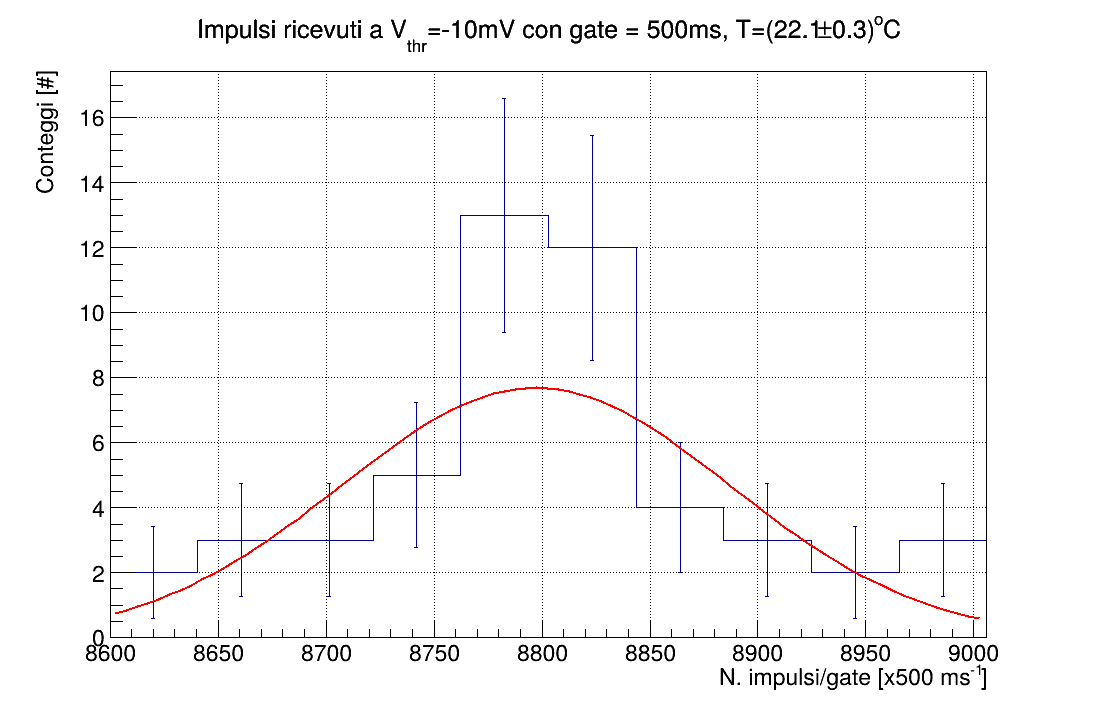
\includegraphics[width=0.99\linewidth]{appendice/dcr_l21.png}
    \caption{\footnotesize $\chi^2=8$, d.o.f.$=7$}
    % 
\end{figure}

\begin{figure}[H]
    \centering
    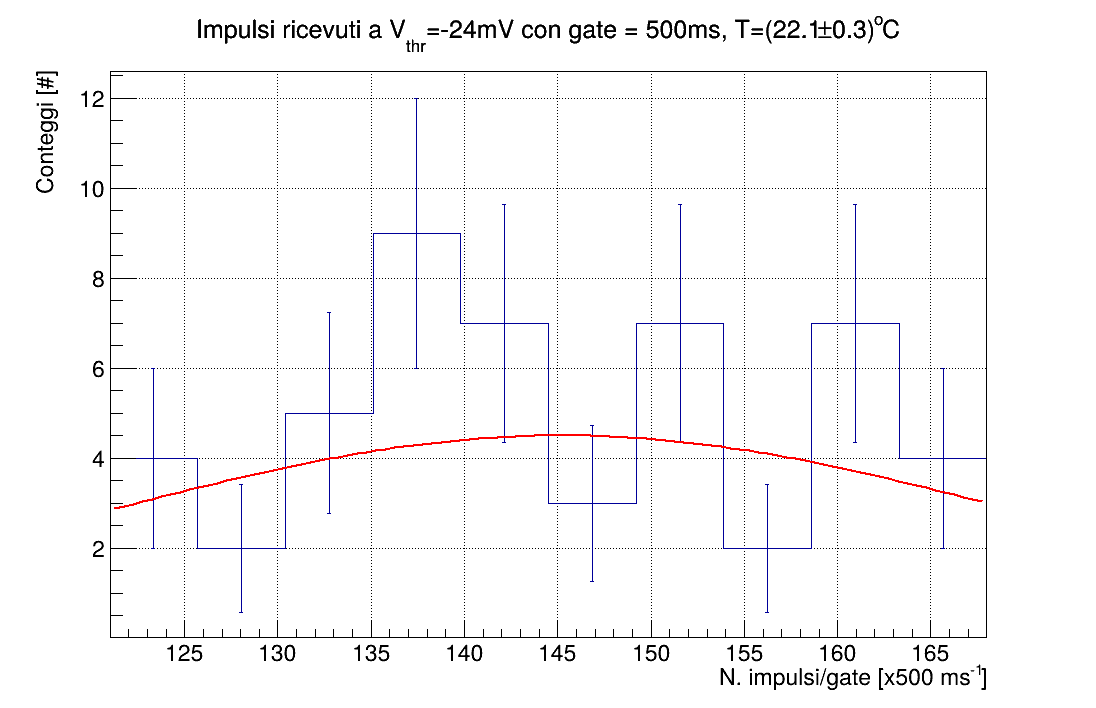
\includegraphics[width=0.99\linewidth]{appendice/dcr_h21.png}
    \caption{\footnotesize $\chi^2=10$, d.o.f.$=7$}
    % 
\end{figure}
\end{multicols}
\begin{multicols}{2}
%33333333333333333333333333333333333333
\begin{figure}[H]
    \centering
    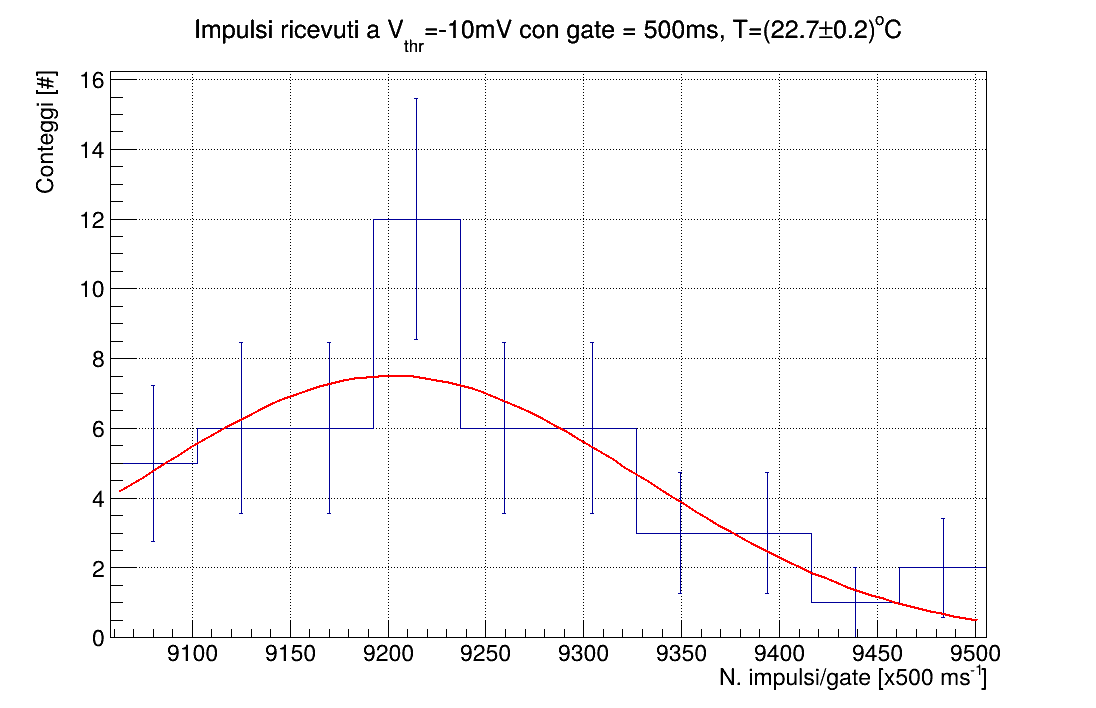
\includegraphics[width=0.99\linewidth]{appendice/dcr_l22.png}
    \caption{\footnotesize $\chi^2=4$, d.o.f.$=7$}
    % 
\end{figure}

\begin{figure}[H]
    \centering
    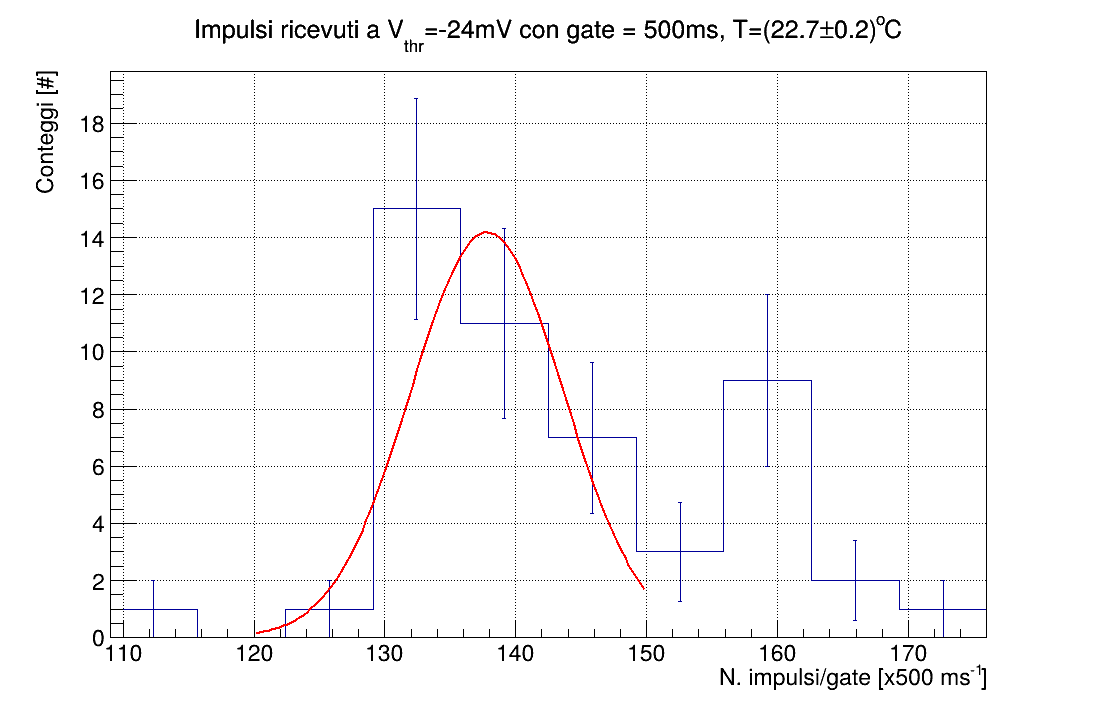
\includegraphics[width=0.99\linewidth]{appendice/dcr_h22.png}
    \caption{\footnotesize $\chi^2=4$, d.o.f.$=1$}
     
\end{figure}
\end{multicols}
\begin{multicols}{2}
%4444444444444444444444444444444444444444444
\begin{figure}[H]
    \centering
    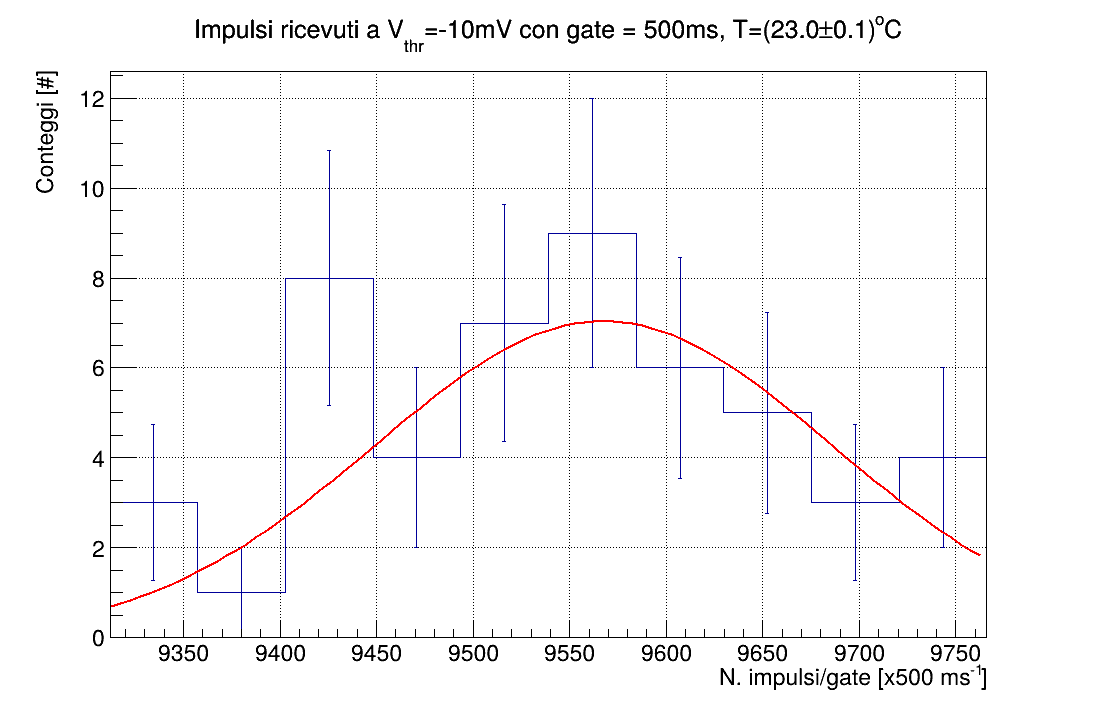
\includegraphics[width=0.99\linewidth]{appendice/dcr_l23.png}
    \caption{\footnotesize $\chi^2=7$, d.o.f.$=7$}
     
\end{figure}

\begin{figure}[H]
    \centering
    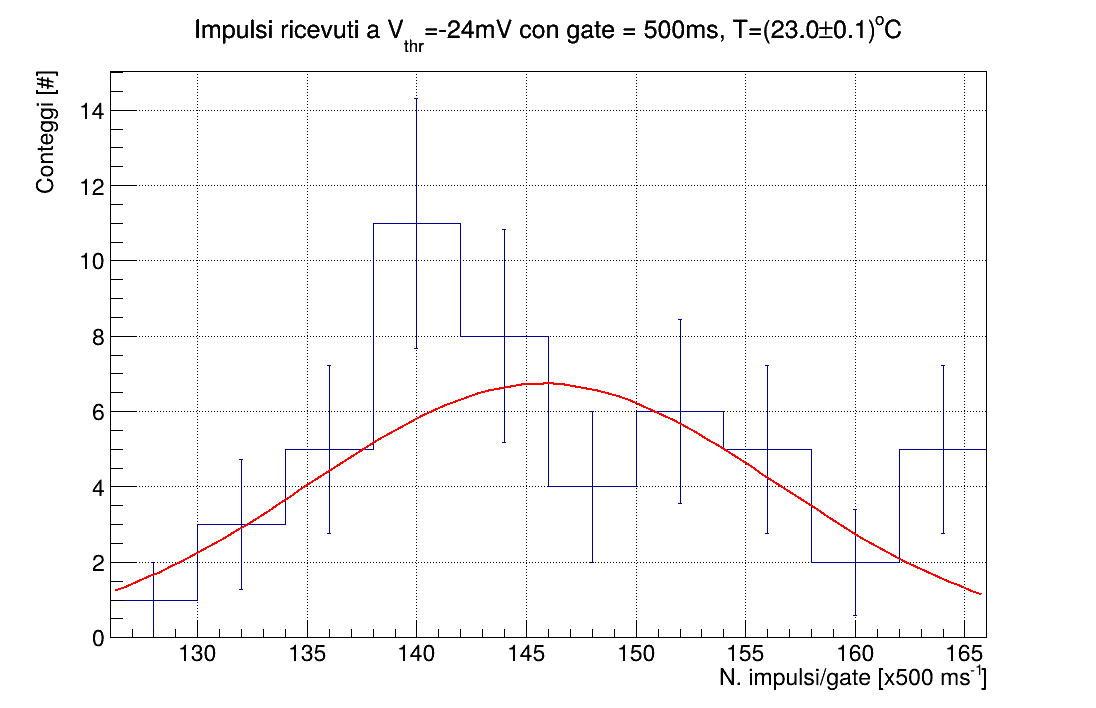
\includegraphics[width=0.99\linewidth]{appendice/dcr_h23.png}
    \caption{\footnotesize $\chi^2=8$, d.o.f.$=7$}
     
\end{figure}
\end{multicols}
\begin{multicols}{2}
%555555555555555555555555555555555555555555555
\begin{figure}[H]
    \centering
    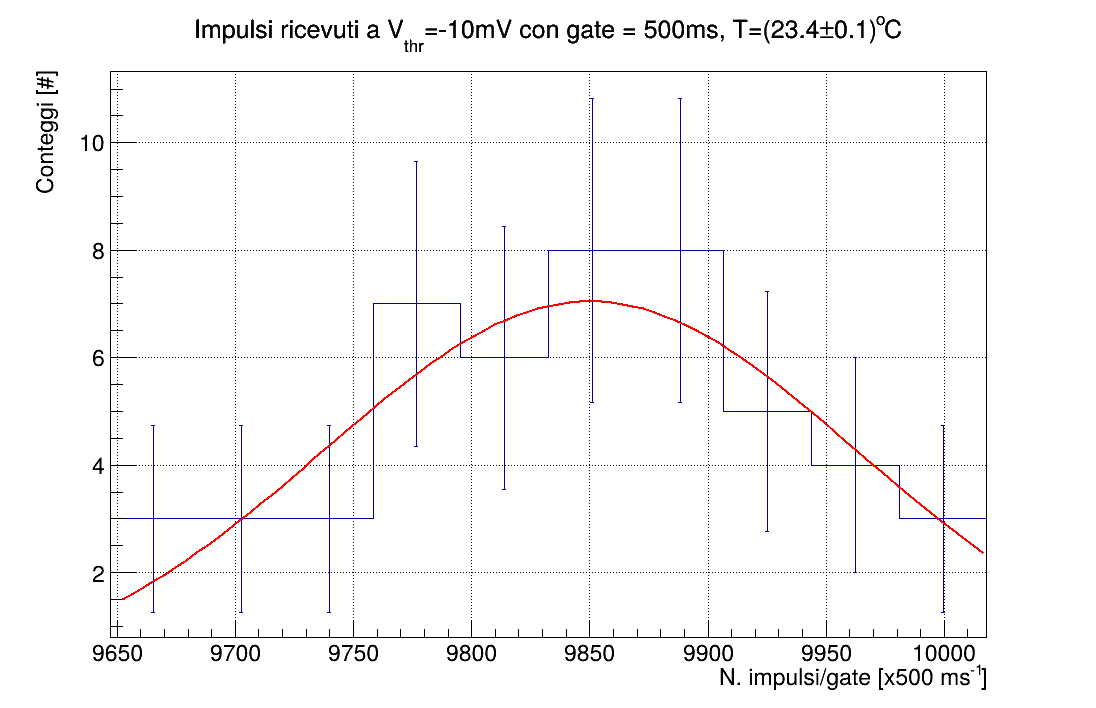
\includegraphics[width=0.99\linewidth]{appendice/dcr_l23_3.png}
    \caption{\footnotesize $\chi^2=2$, d.o.f.$=7$}
     
\end{figure}

\begin{figure}[H]
    \centering
    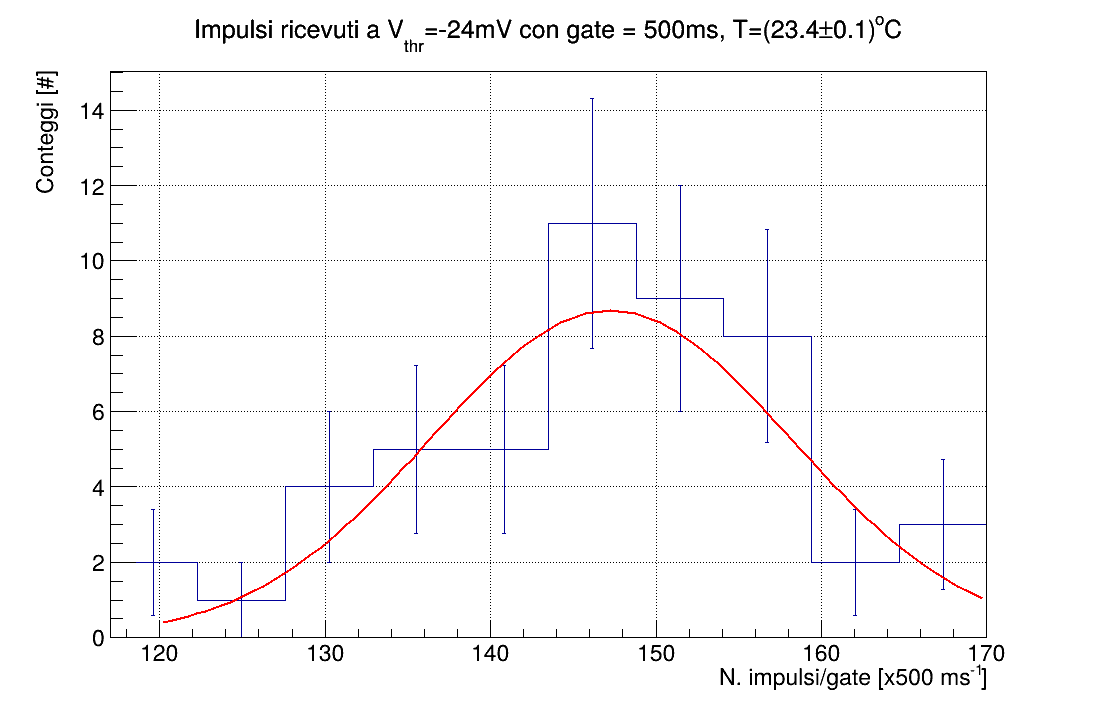
\includegraphics[width=0.99\linewidth]{appendice/dcr_h23_3.png}
    \caption{\footnotesize $\chi^2=4$, d.o.f.$=6$}
     
\end{figure}
\end{multicols}
\begin{multicols}{2}
%66666666666666666666666666666666666666666666666
\begin{figure}[H]
    \centering
    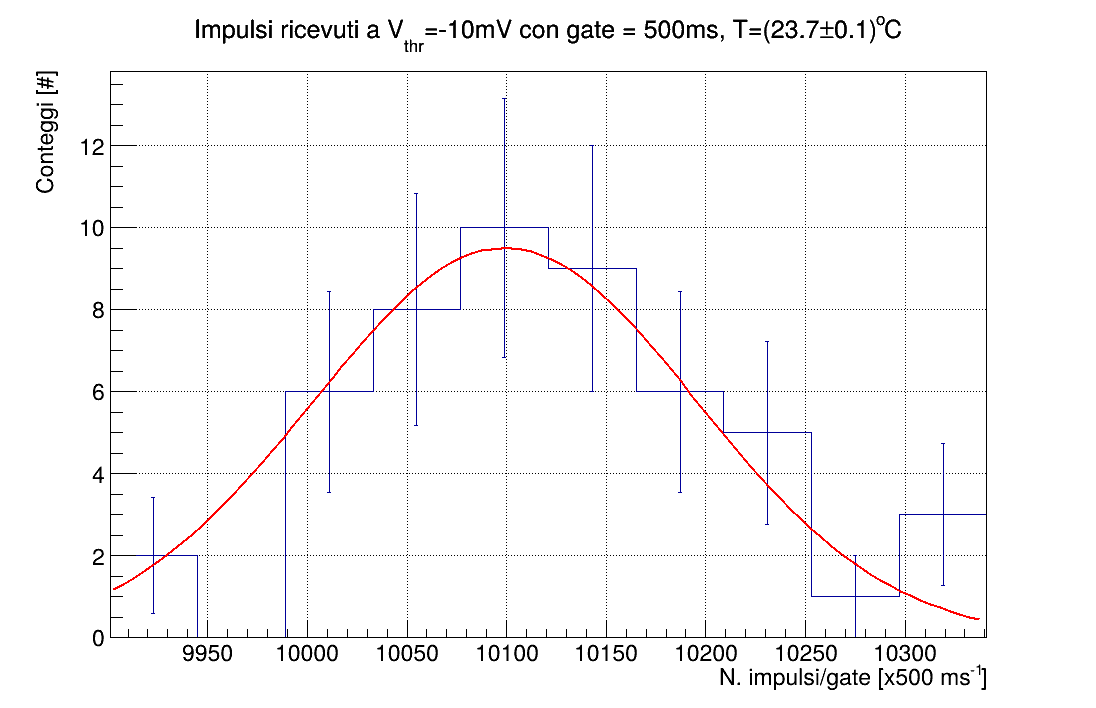
\includegraphics[width=0.99\linewidth]{appendice/dcr_l23_6.png}
    \caption{\footnotesize $\chi^2=3$, d.o.f.$=6$}
     
\end{figure}

\begin{figure}[H]
    \centering
    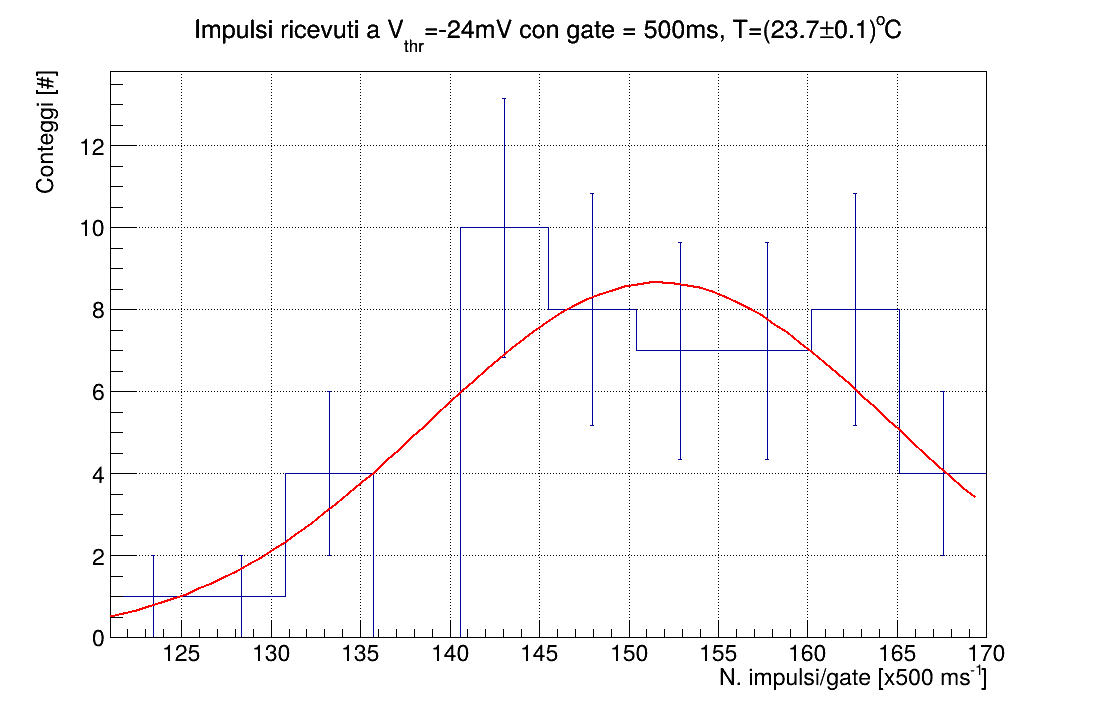
\includegraphics[width=0.99\linewidth]{appendice/dcr_h23_6.png}
    \caption{\footnotesize $\chi^2=3$, d.o.f.$=6$}
     
\end{figure}
\end{multicols}
\newpage
\begin{multicols}{2}
%777777777777777777777777777777777777777777777777
\begin{figure}[H]
    \centering
    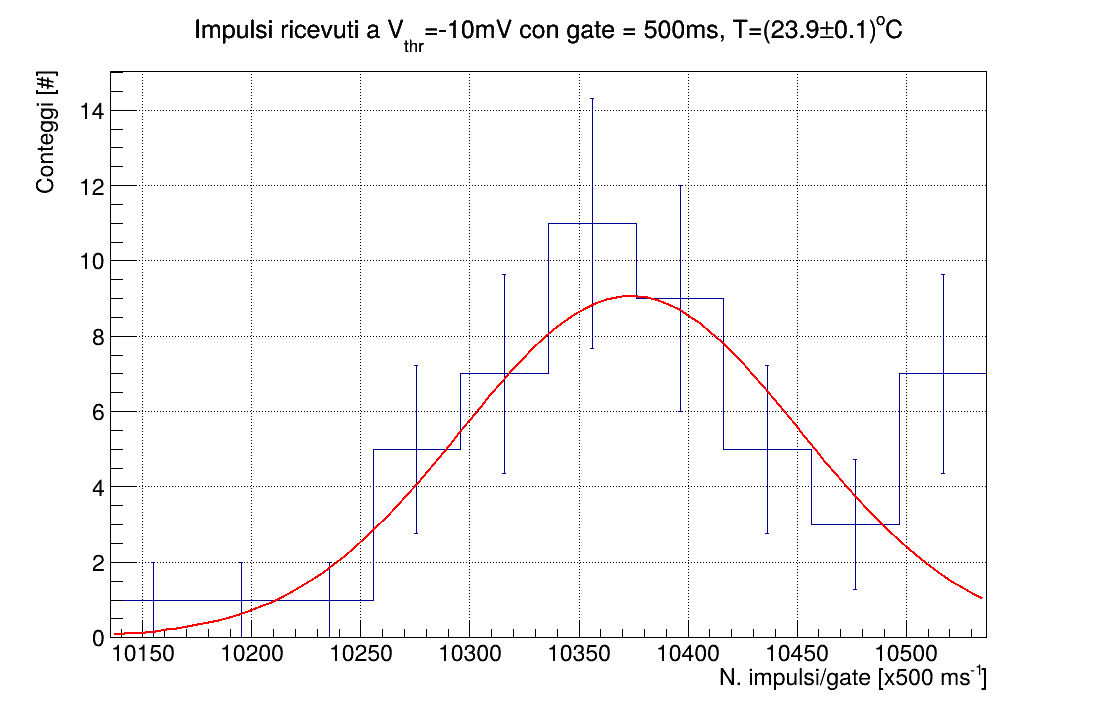
\includegraphics[width=0.99\linewidth]{appendice/dcr_l23_9.png}
    \caption{\footnotesize $\chi^2=7$, d.o.f.$=7$}
     
\end{figure}

\begin{figure}[H]
    \centering
    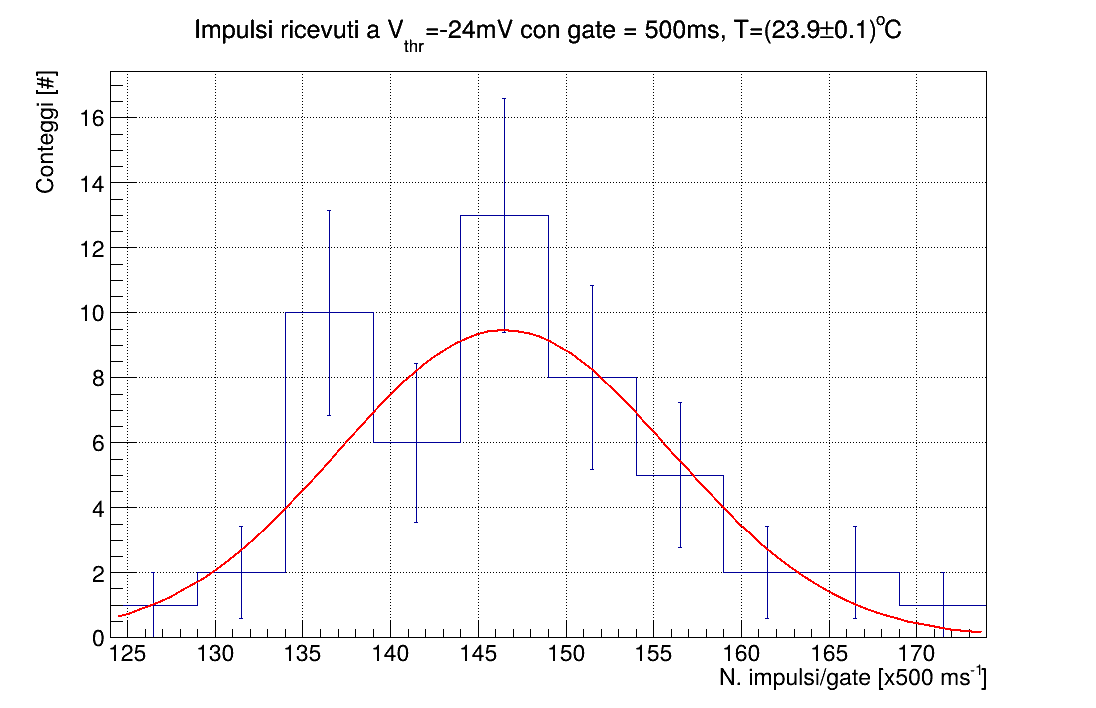
\includegraphics[width=0.99\linewidth]{appendice/dcr_h23_9.png}
    \caption{\footnotesize $\chi^2=5$, d.o.f.$=7$}
     
\end{figure}
\end{multicols}

\subsection{Caratterizzazione di un SiPM con sorgente luminosa (LED)}
\subsubsection{Stima di $G_{SiPM}$}
Si riportano qui i valori dei picchi della sezione 1.2.1, le loro incertezze e le stime di $\Delta_{pp}$.

\begin{table}[H]
    \centering
    \begin{tabular}{|c|c|c|c|c|}
        \hline
        
        \textbf{N. picco} & \textbf{$\mathbf{\chi^2}$ fit} & \textbf{d.o.f.} &$\mathbf{(p_i\pm\sigma_{p,i})}$\textbf{[CHN]} & $\mathbf{\Delta_{pp}}$\textbf{[CHN]} \\ \hline
        
        0   & 27 & 27 & $1\pm8$ & \textbf{X} \\ \hline
        1   & 40 & 52 & $233\pm12$    & $232\pm15$ \\ \hline
        2   & 72 & 71 & $463\pm17$    & $230\pm20$ \\ \hline        
        3   & 100 & 82 & $690\pm20$   & $230\pm30$ \\ \hline
        4   & 96 & 97 & $920\pm30$    & $230\pm40$ \\ \hline
        5   & 141 & 117 & $1150\pm40$ & $230\pm50$ \\ \hline
    \end{tabular}
    \caption{\footnotesize Coordinate dei picchi, parametri dei fit e stime di $\Delta_{pp}$ utilizzate per il calcolo di $G_{SiPM}$.}
    \label{tab:gsipm}   
\end{table}
\subsubsection{$\Delta_{pp}$ in funzione di $G_{ampl}$}
\label{sec:app_gain}
Si riportano qui gli spettri del LED al variare di $G_{ampl}$, usati nella sezione 1.2.2.
\begin{multicols}{2}
    \begin{figure}[H]
    \centering
    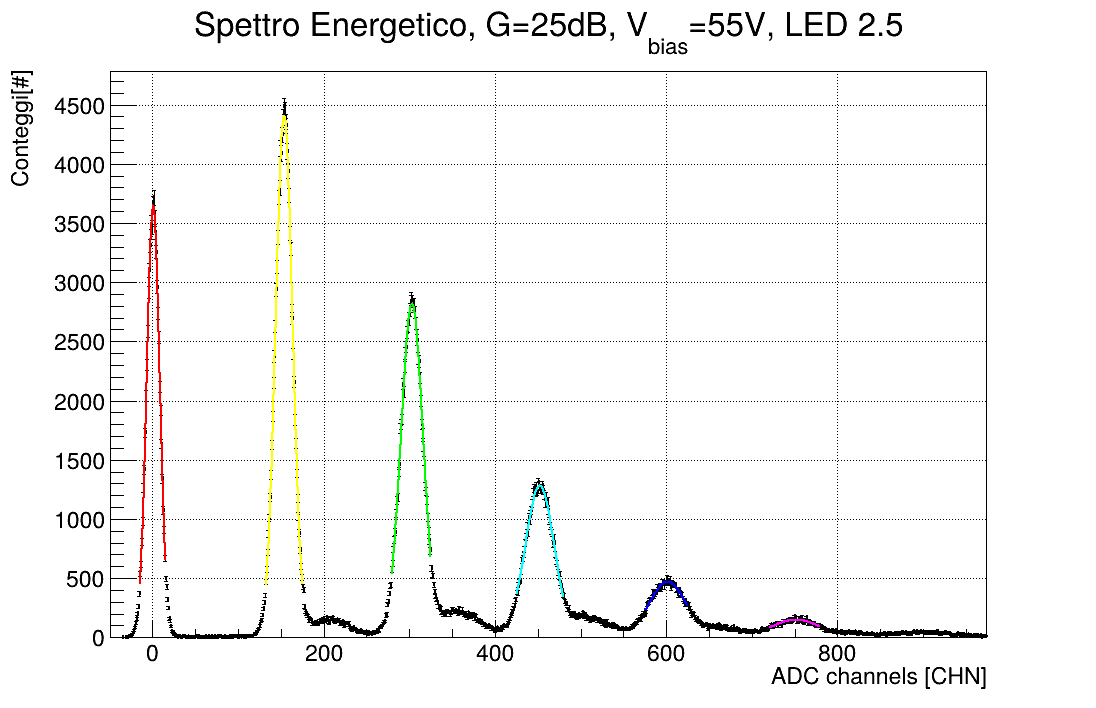
\includegraphics[width=0.99\linewidth]{appendice/gain25.png}
     
\end{figure}
\begin{figure}[H]
    \centering
    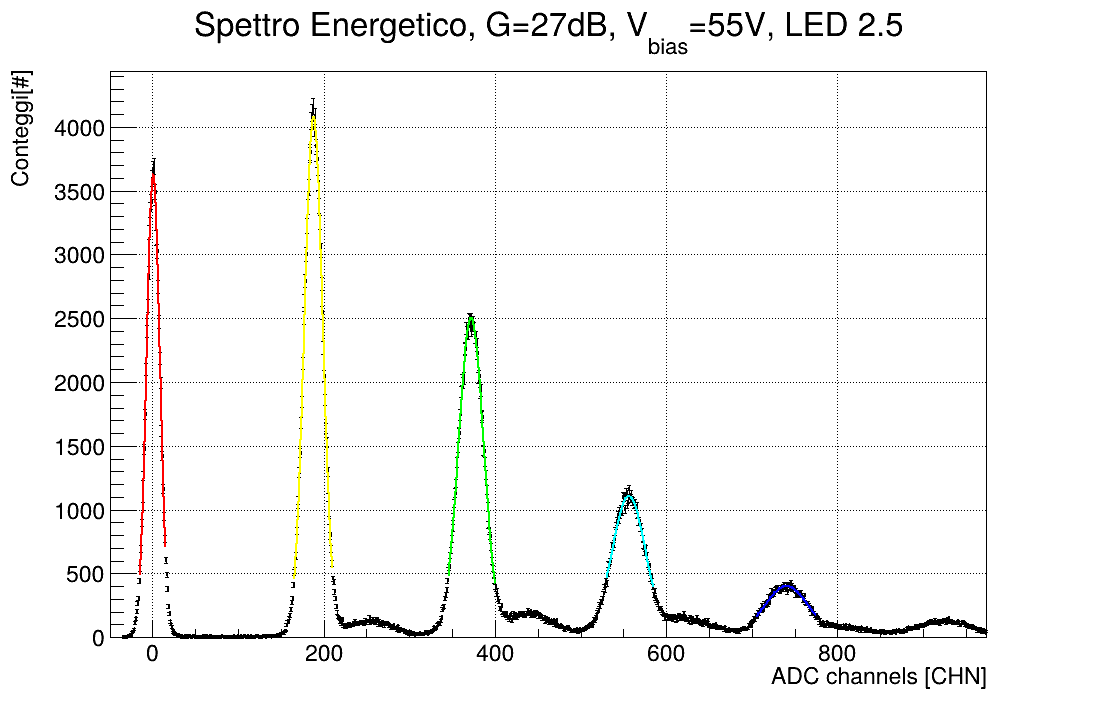
\includegraphics[width=0.99\linewidth]{appendice/gain27.png}
     
\end{figure}
\end{multicols}
\newpage
\begin{multicols}{2}
    \begin{figure}[H]
    \centering
    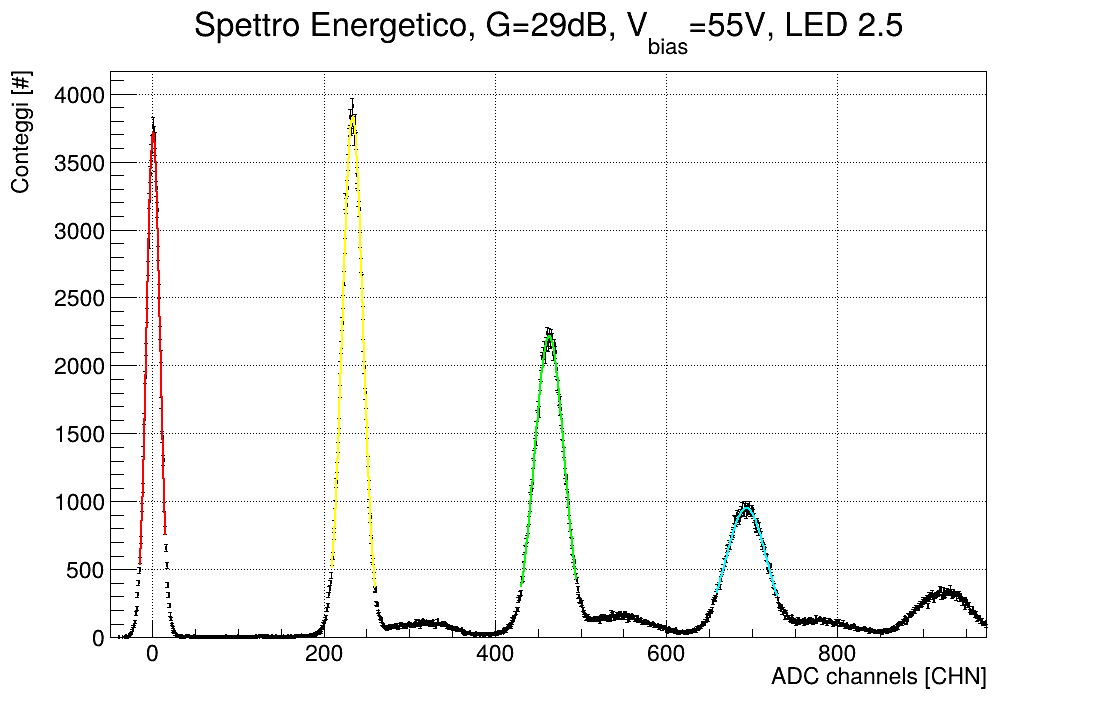
\includegraphics[width=0.99\linewidth]{appendice/gain29.png}
     
\end{figure}
\begin{figure}[H]
    \centering
    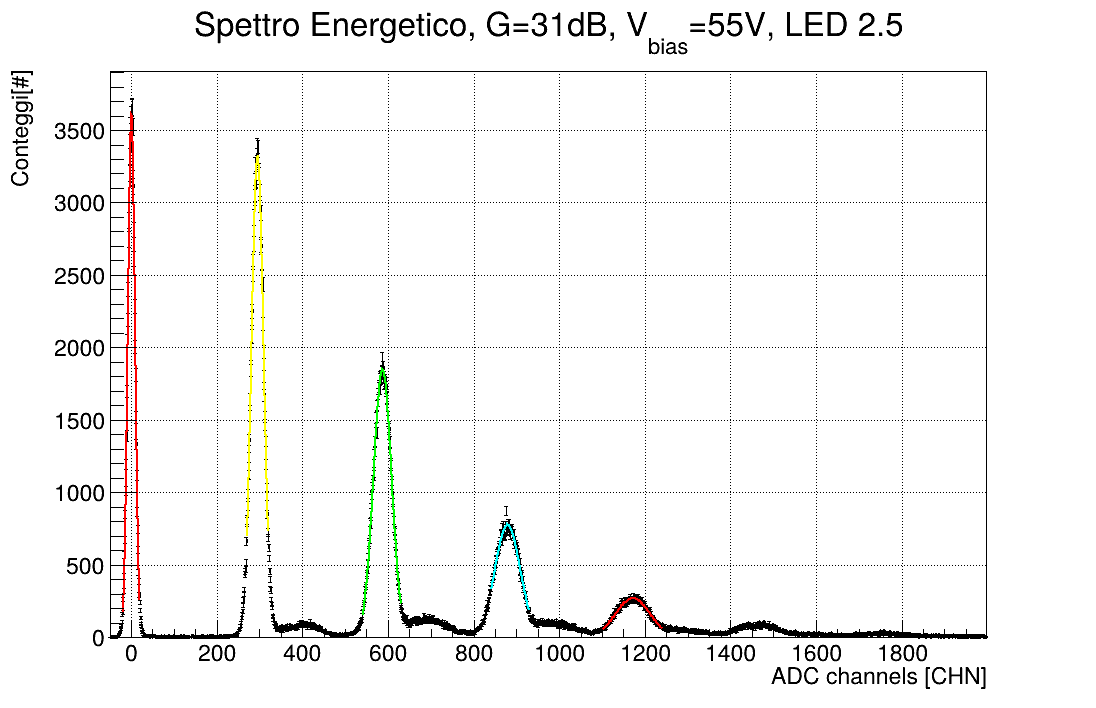
\includegraphics[width=0.99\linewidth]{appendice/gain31.png}
     
\end{figure}
\end{multicols}

\begin{multicols}{2}
    \begin{figure}[H]
    \centering
    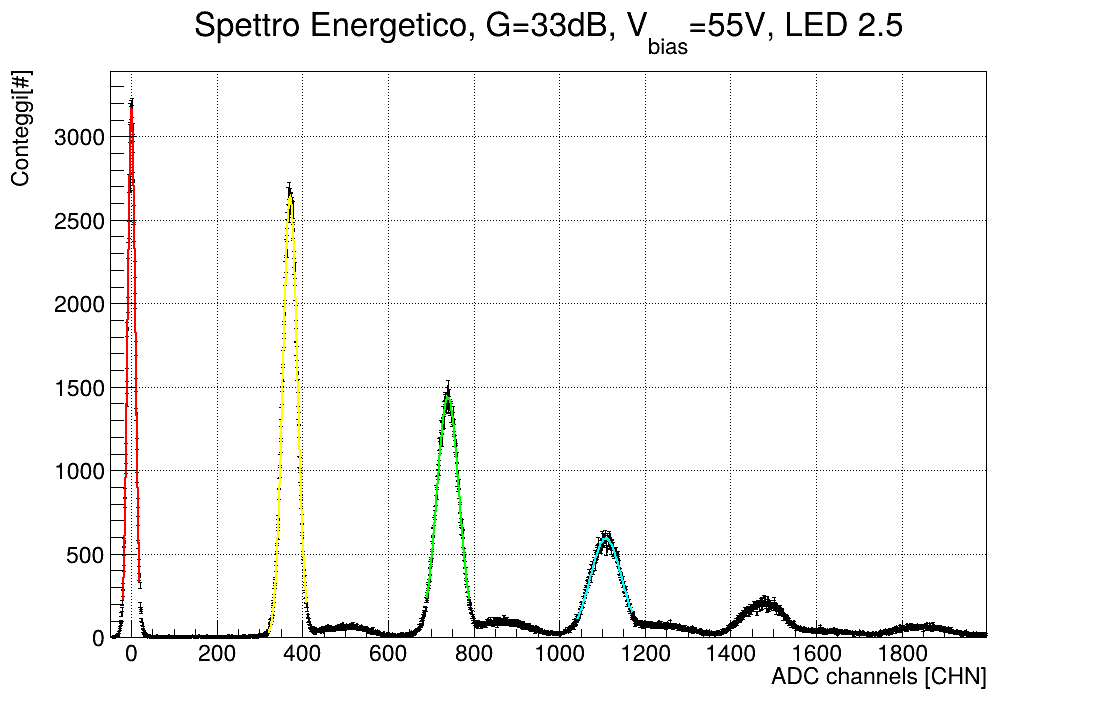
\includegraphics[width=0.99\linewidth]{appendice/gain33.png}
     
\end{figure}
\begin{figure}[H]
    \centering
    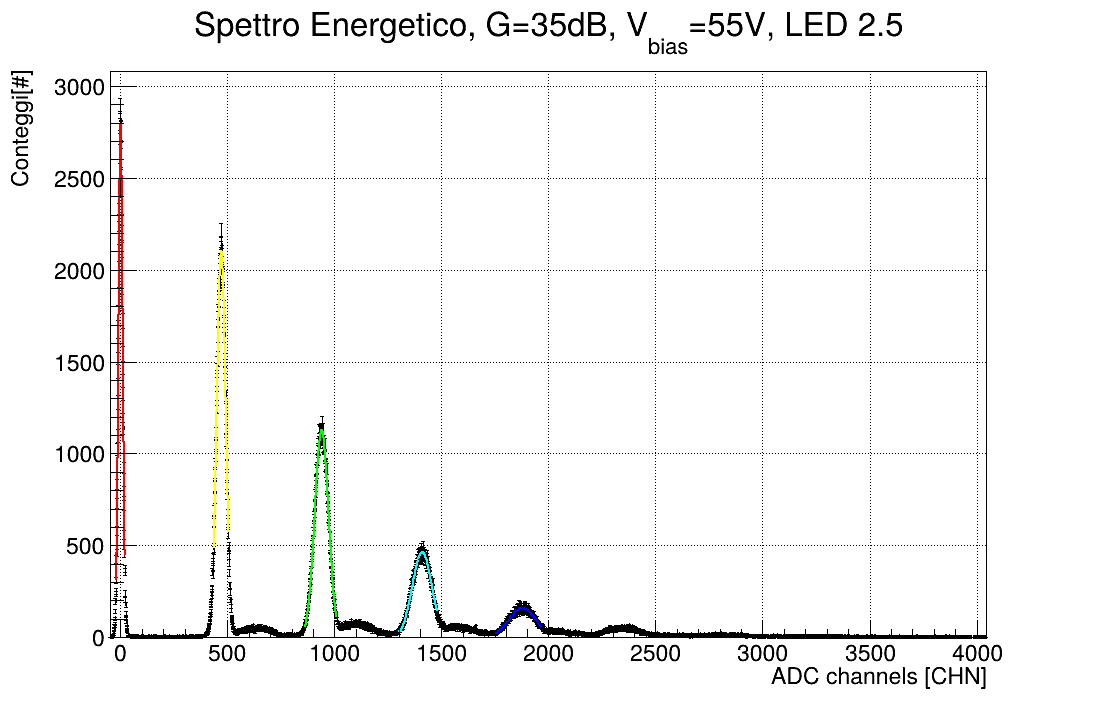
\includegraphics[width=0.99\linewidth]{appendice/gain35.png}
     
\end{figure}
\end{multicols}
\subsubsection{$G_{SiPM}$ in funzione di $V_{bias}$}
Si riportano qui gli spettri del LED al variare di $V_{bias}$, usati nella sezione 1.2.3.
\begin{multicols}{2}
    \begin{figure}[H]
    \centering
    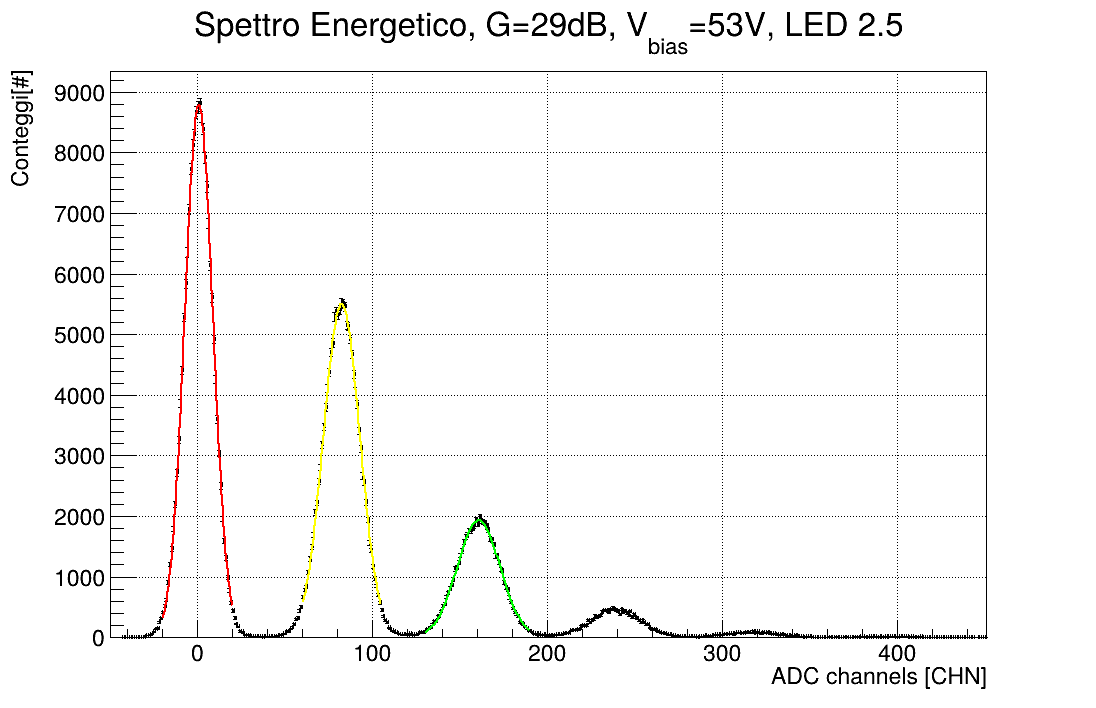
\includegraphics[width=0.99\linewidth]{appendice/V53.png}
     
\end{figure}
\begin{figure}[H]
    \centering
    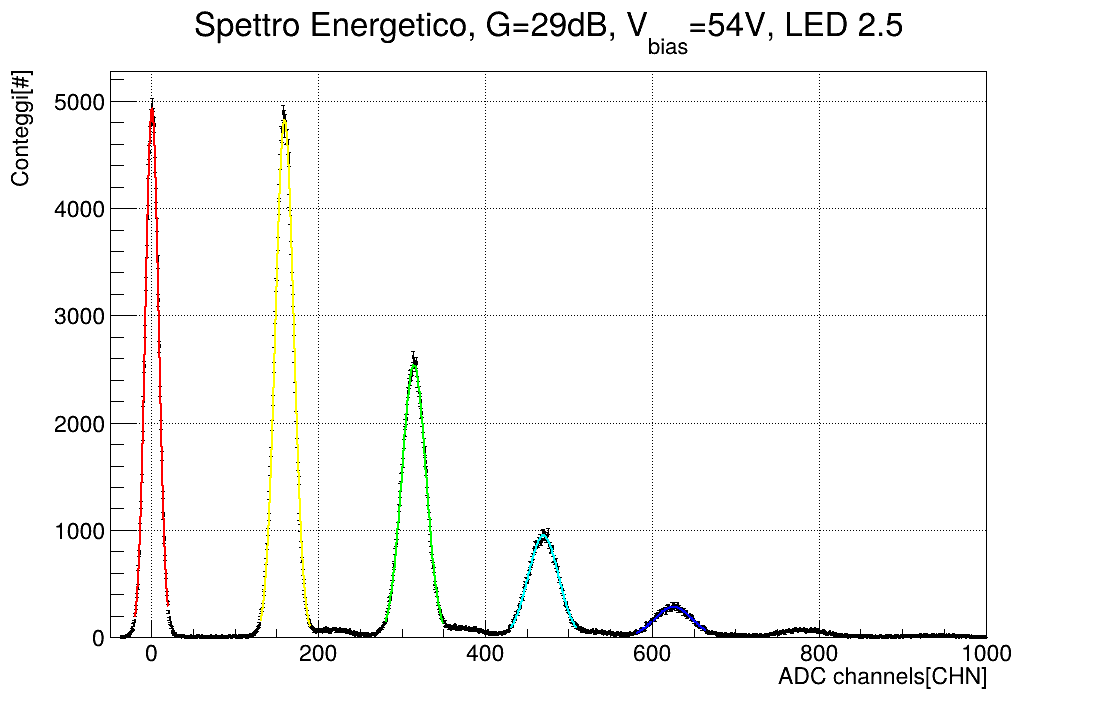
\includegraphics[width=0.99\linewidth]{appendice/V54.png}
     
\end{figure}
\end{multicols}
\newpage
\begin{multicols}{2}
    \begin{figure}[H]
    \centering
    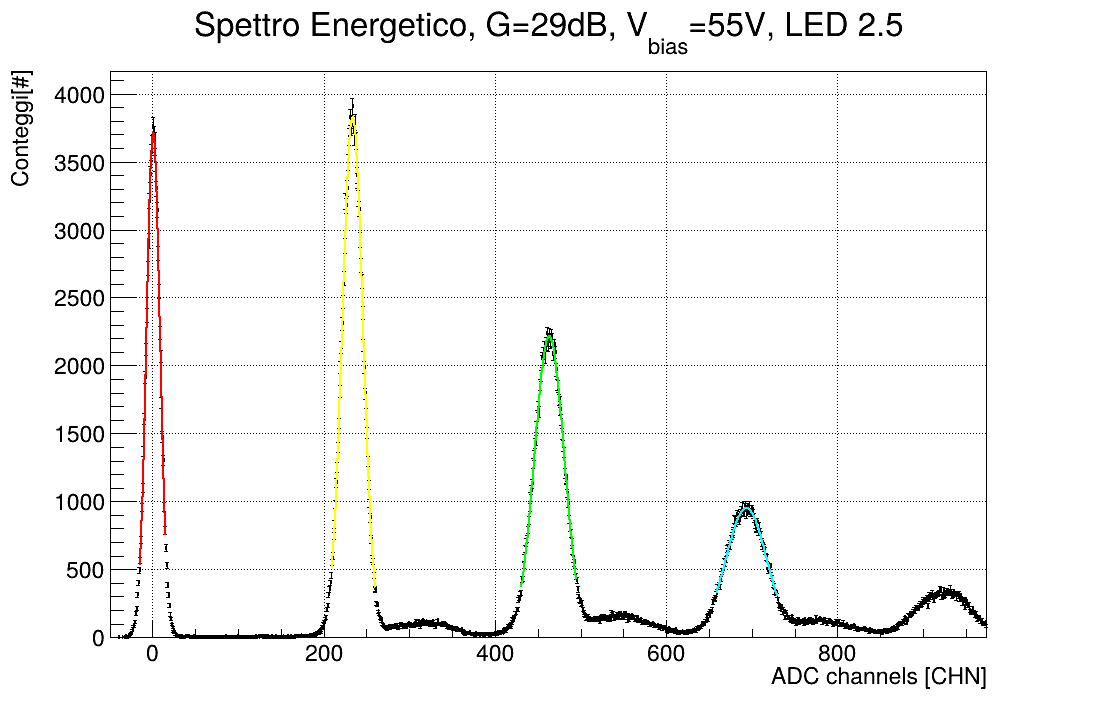
\includegraphics[width=0.99\linewidth]{appendice/V55.png}
     
\end{figure}
\begin{figure}[H]
    \centering
    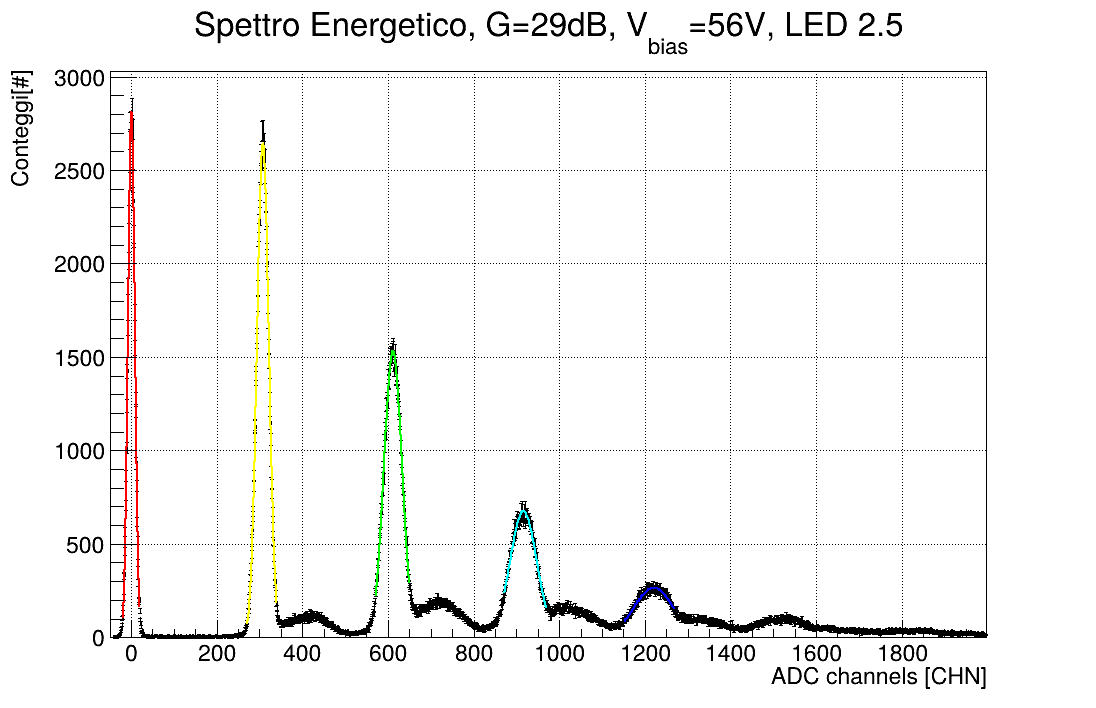
\includegraphics[width=0.99\linewidth]{appendice/V56.png}
     
\end{figure}
\end{multicols}
\begin{multicols}{2}
\begin{figure}[H]
    \centering
    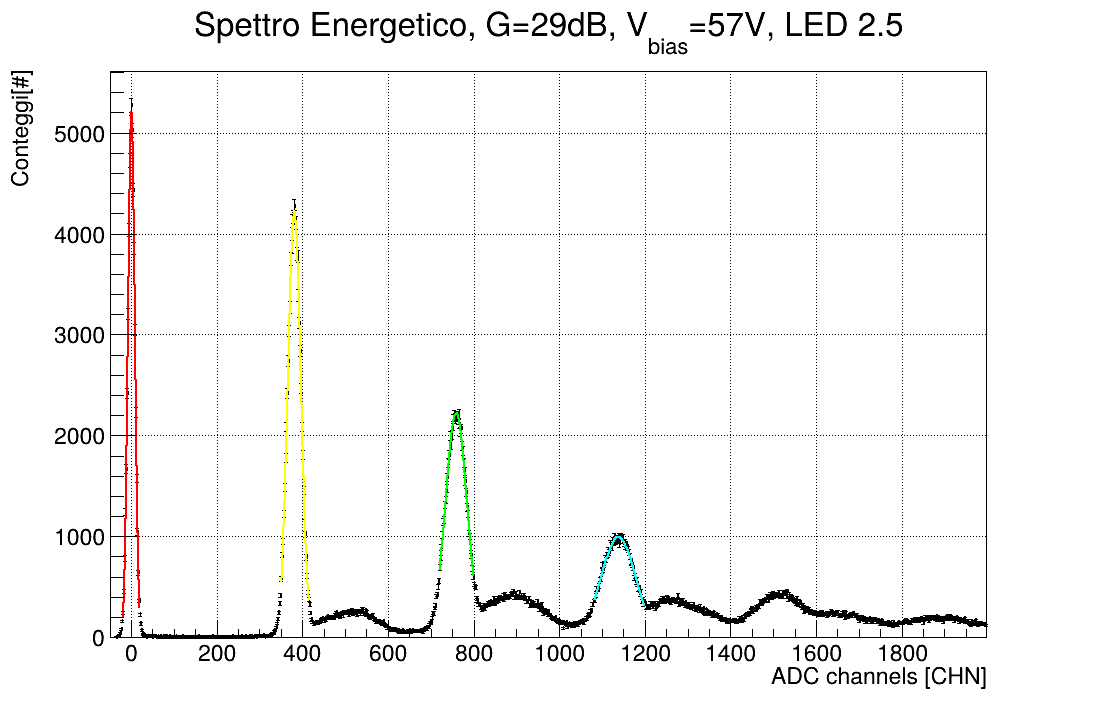
\includegraphics[width=0.99\linewidth]{appendice/V57.png}
     
\end{figure}
\end{multicols}
\subsubsection{Stima del numero di fotoni rivelati}

Si riportano qui i valori dei picchi della sezione 1.2.4 ($I_{LED} = 2.5$), le loro incertezze e le stime di $\Delta_{pp}$.

\begin{table}[H]
    \centering
    \begin{tabular}{|c|c|c|c|c|}
        \hline
        
        \textbf{N. picco} & \textbf{$\mathbf{\chi^2}$ fit} & \textbf{d.o.f.} &$\mathbf{(p_i\pm\sigma_{p,i})}$\textbf{[CHN]} & $\mathbf{\Delta_{pp}}$\textbf{[CHN]} \\ \hline
        
        0   & 46 & 37 & $1\pm8$ & \textbf{X} \\ \hline
        1   & 65 & 52 & $234\pm12$    & $232\pm15$ \\ \hline
        2   & 67 & 72 & $463\pm17$    & $230\pm20$ \\ \hline        
        3   & 71 & 77 & $690\pm20$   & $230\pm30$ \\ \hline
    \end{tabular}
    \caption{\footnotesize Coordinate dei picchi, parametri dei fit e stime di $\Delta_{pp}$ utilizzate per il calcolo di $\mu_{ph}$ a $I_{LED} = 2.5$}
    \label{tab:led2_5}   
\end{table}
\newpage
Si riportano gli spettri con $I_{LED} = 2.0$ e $2.8$
\begin{multicols}{2}
    \begin{figure}[H]
    \centering
    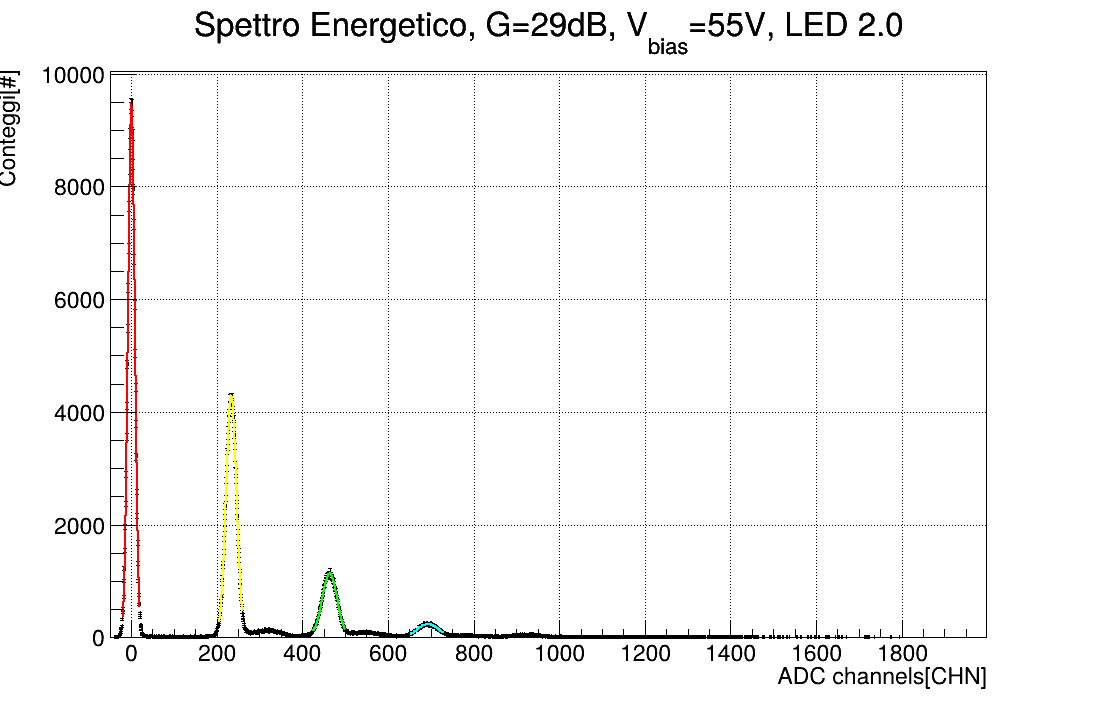
\includegraphics[width=0.99\linewidth]{appendice/i2_0.png}
     
\end{figure}
\begin{figure}[H]
    \centering
    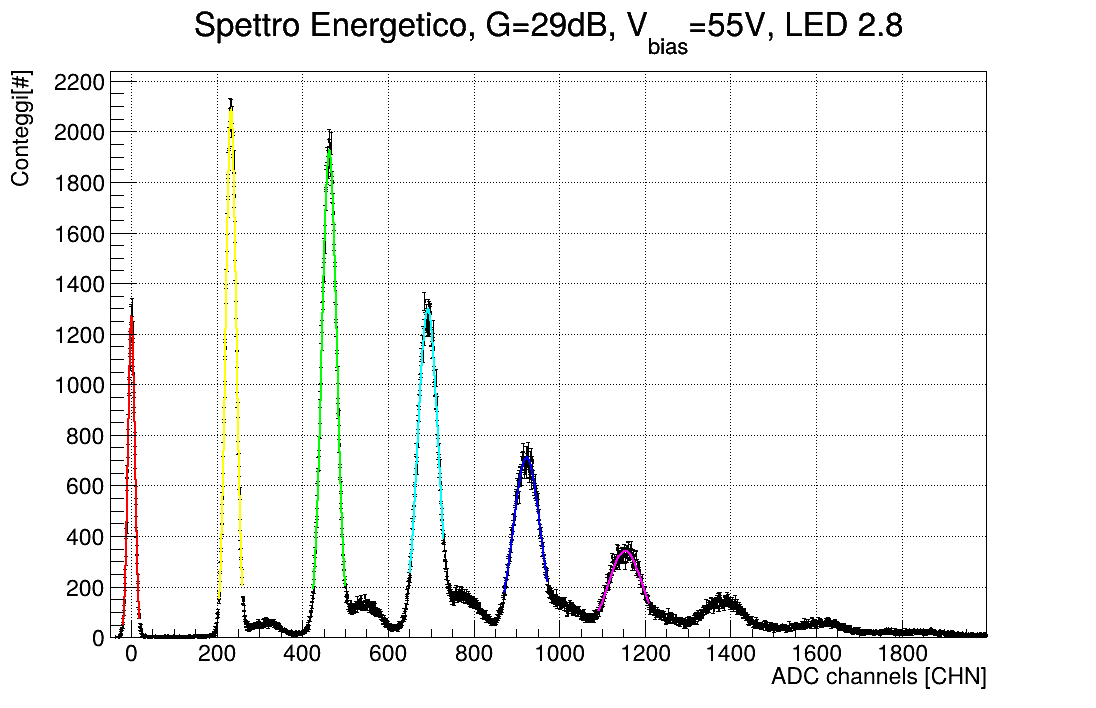
\includegraphics[width=0.99\linewidth]{appendice/i2_8.png}
     
\end{figure}
\end{multicols}

Si riportano gli istogrammi delle aree sottese e i grafici $\sigma^2_N$ vs N.

\begin{multicols}{2}
    \begin{figure}[H]
    \centering
    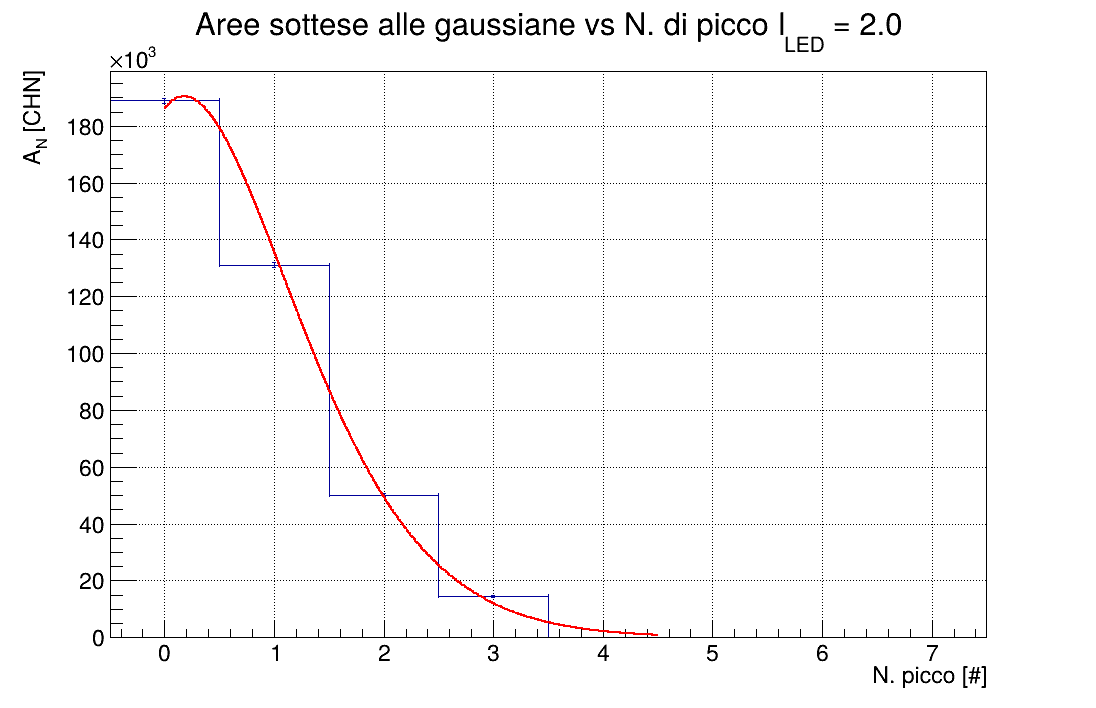
\includegraphics[width=0.99\linewidth]{appendice/pois2_0.png}
    \caption{ \footnotesize $\chi^2 = 93$, d.o.f$=2$.}
     
\end{figure}
\begin{figure}[H]
    \centering
    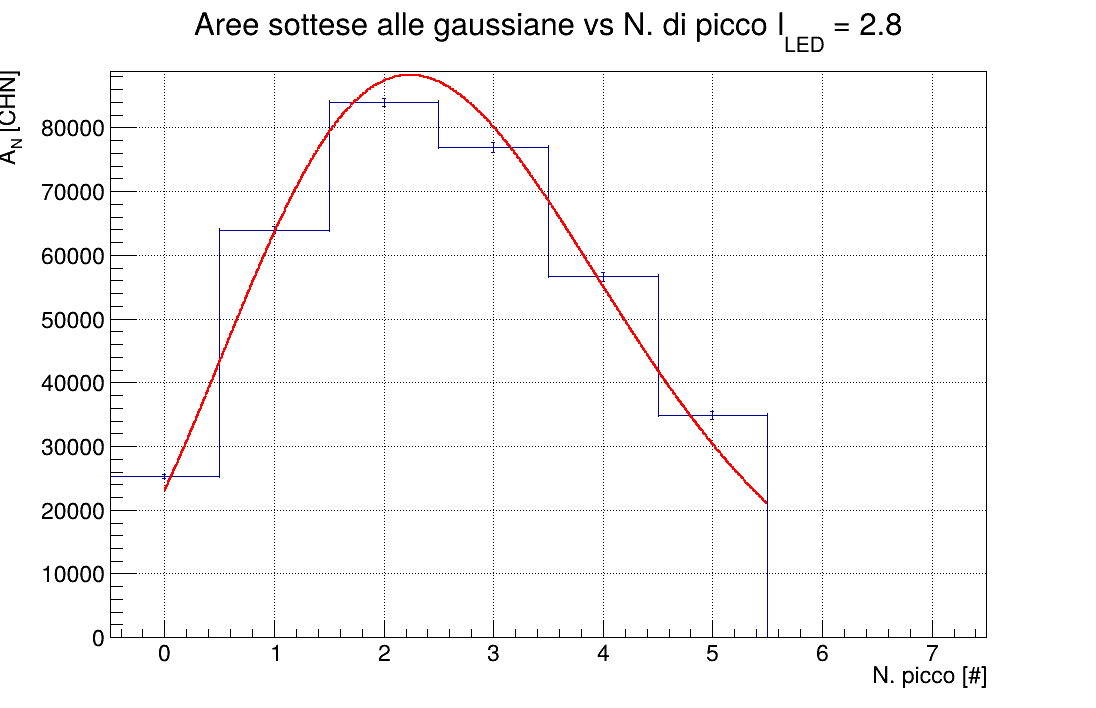
\includegraphics[width=0.99\linewidth]{appendice/pois2_8.png}
    \caption{ \footnotesize $\chi^2 = 143$, d.o.f$=4$.}
     
\end{figure}
\end{multicols}
\begin{multicols}{2}
    \begin{figure}[H]
    \centering
    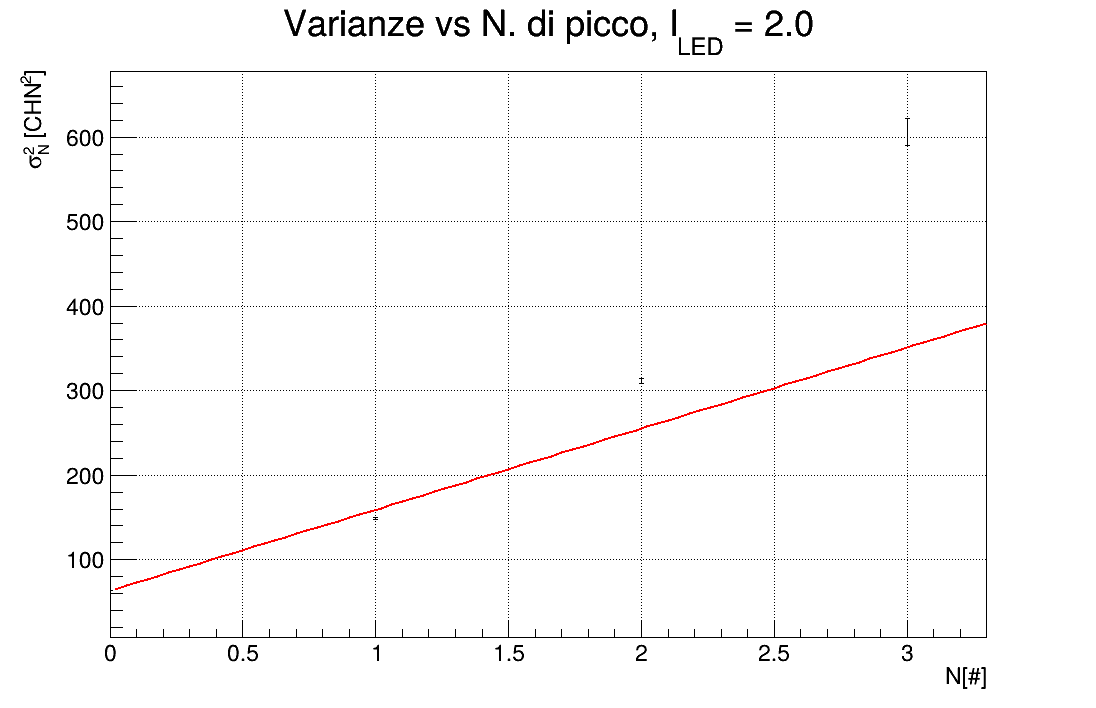
\includegraphics[width=0.99\linewidth]{appendice/sigma2_0.png}
    \caption{ \footnotesize  $\chi^2 = 3379$, d.o.f$=4$.}
     
\end{figure}
\begin{figure}[H]
    \centering
    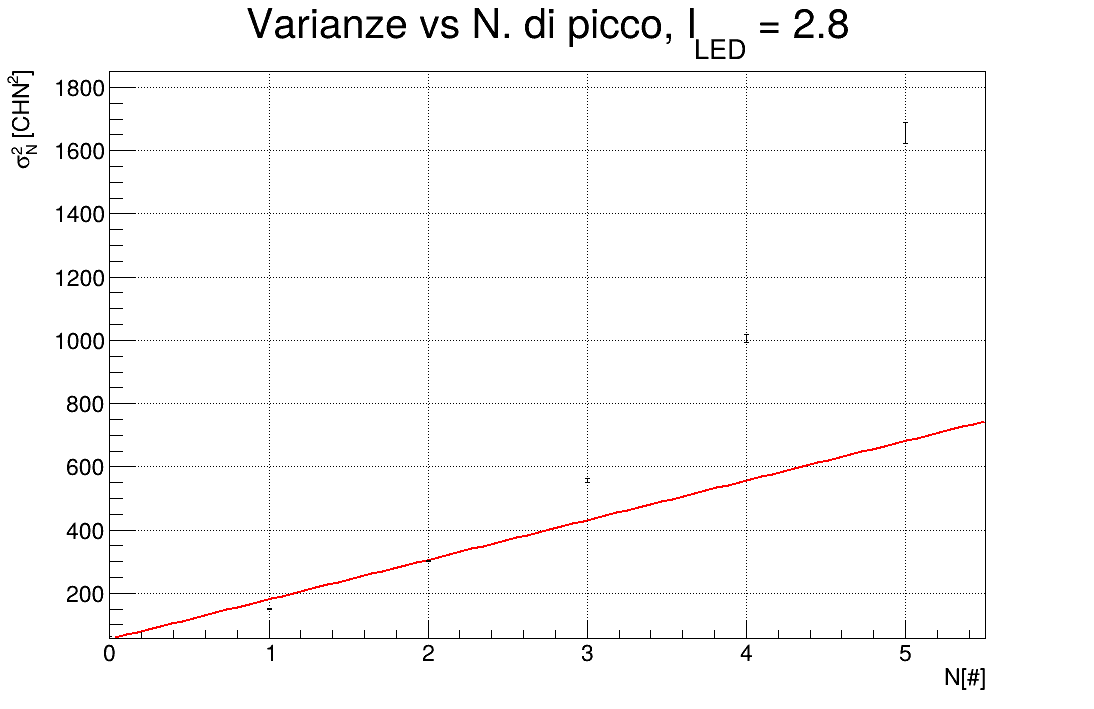
\includegraphics[width=0.99\linewidth]{appendice/sigma2_8.png}
    \caption{ \footnotesize $\chi^2 = 143$, d.o.f$=4$.}
     
\end{figure}
\end{multicols}
\newpage
\subsection{Istogrammi assorbimento $\beta^-$
}
Vengono qui riportati gli istogrammi per l'analisi dell'assorbimento con sorgente di $^{90}Sr$ relativi alla sezione 2.2.1 e 2.2.2 con i relativi fit gaussiani.

\subsubsection{Istogrammi per carta}

\begin{multicols}{2}
    \begin{figure}[H]
    \centering
    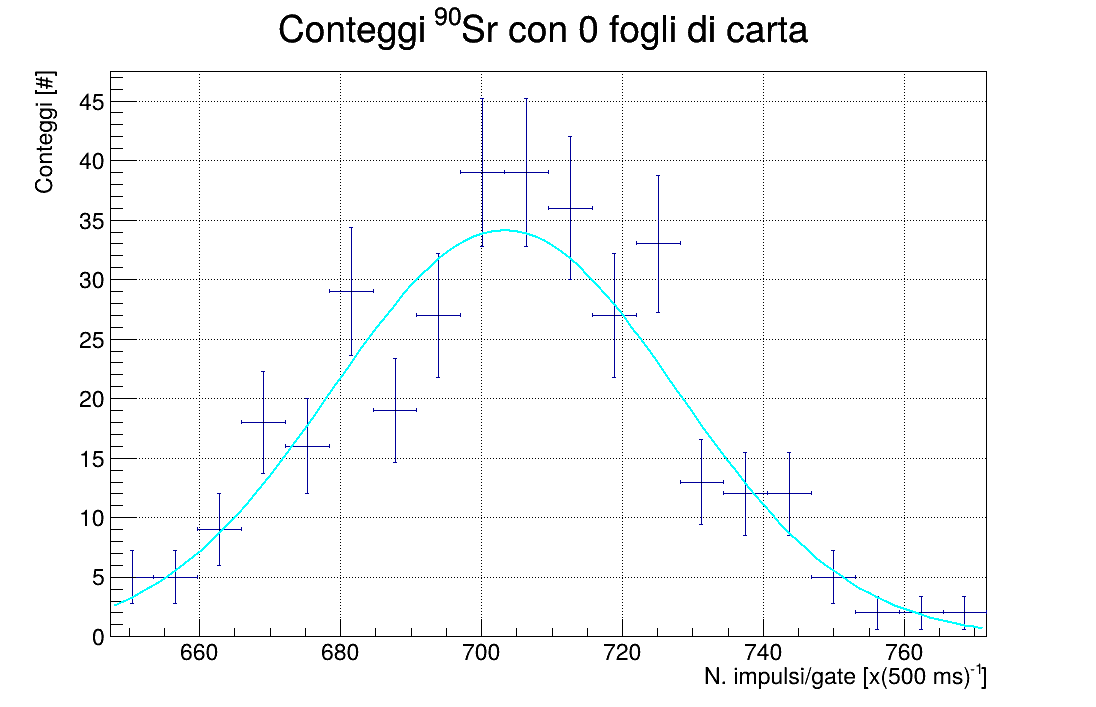
\includegraphics[width=0.99\linewidth]{appendice/carta/c0.png}
    \caption{\footnotesize $\chi^2=17$, d.o.f.$=17$}
     
\end{figure}
\begin{figure}[H]
    \centering
    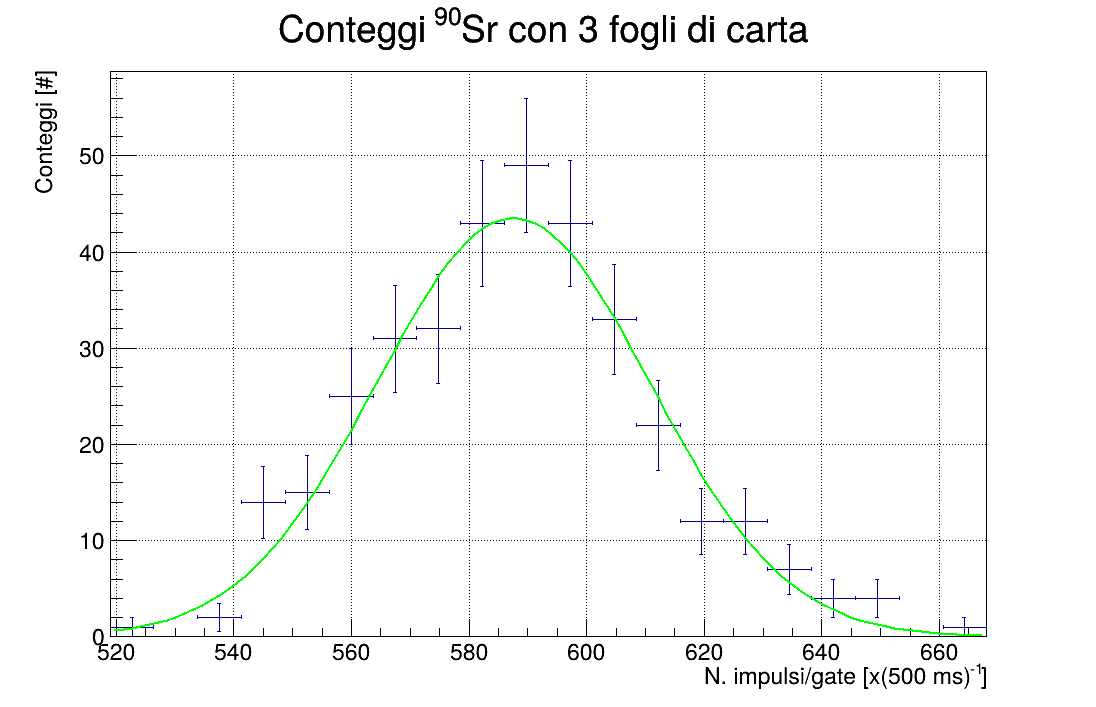
\includegraphics[width=0.99\linewidth]{appendice/carta/c1.png}
    \caption{\footnotesize $\chi^2=13$, d.o.f.$=15$}
     
\end{figure}
\end{multicols}
\begin{multicols}{2}
    \begin{figure}[H]
    \centering
    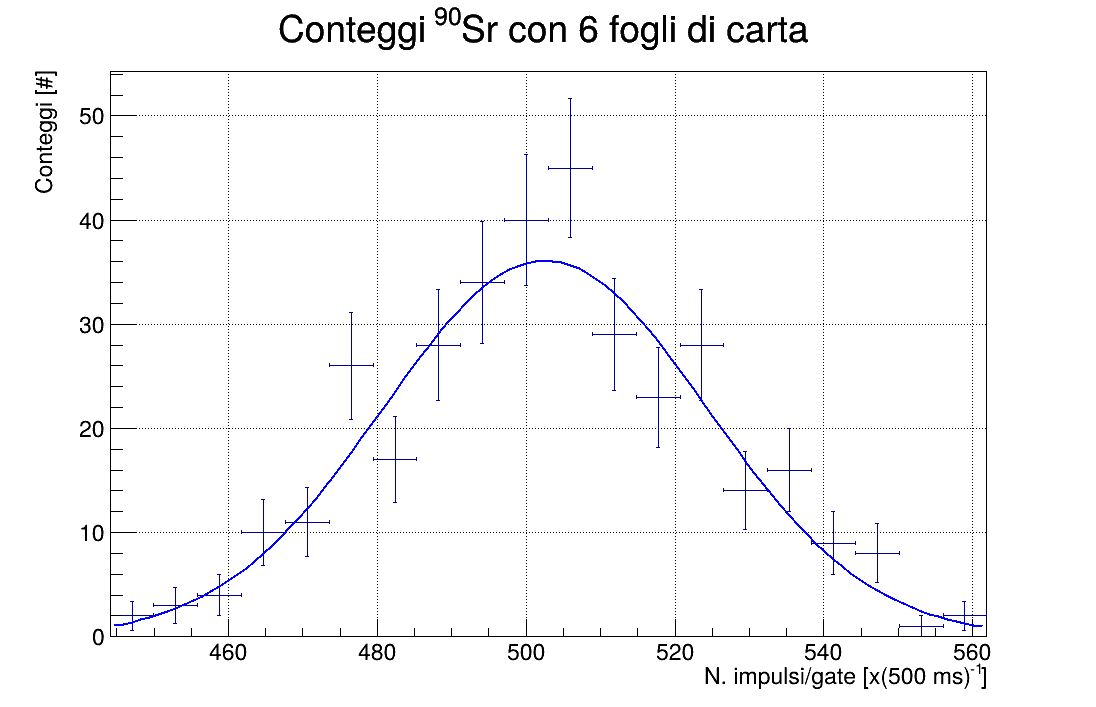
\includegraphics[width=0.99\linewidth]{appendice/carta/c2.png}
    \caption{\footnotesize $\chi^2=17$, d.o.f.$=17$}
     
\end{figure}
\begin{figure}[H]
    \centering
    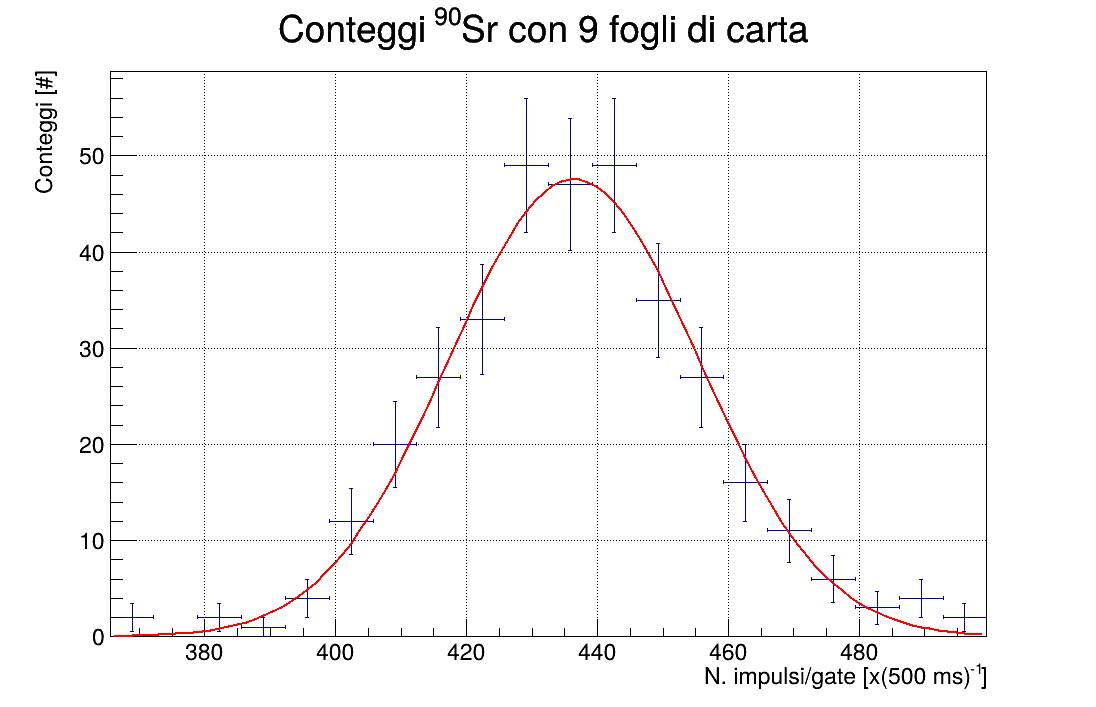
\includegraphics[width=0.99\linewidth]{appendice/carta/c3.png}
    \caption{\footnotesize $\chi^2=10$, d.o.f.$=16$}
     
\end{figure}
\end{multicols}
\begin{multicols}{2}
    \begin{figure}[H]
    \centering
    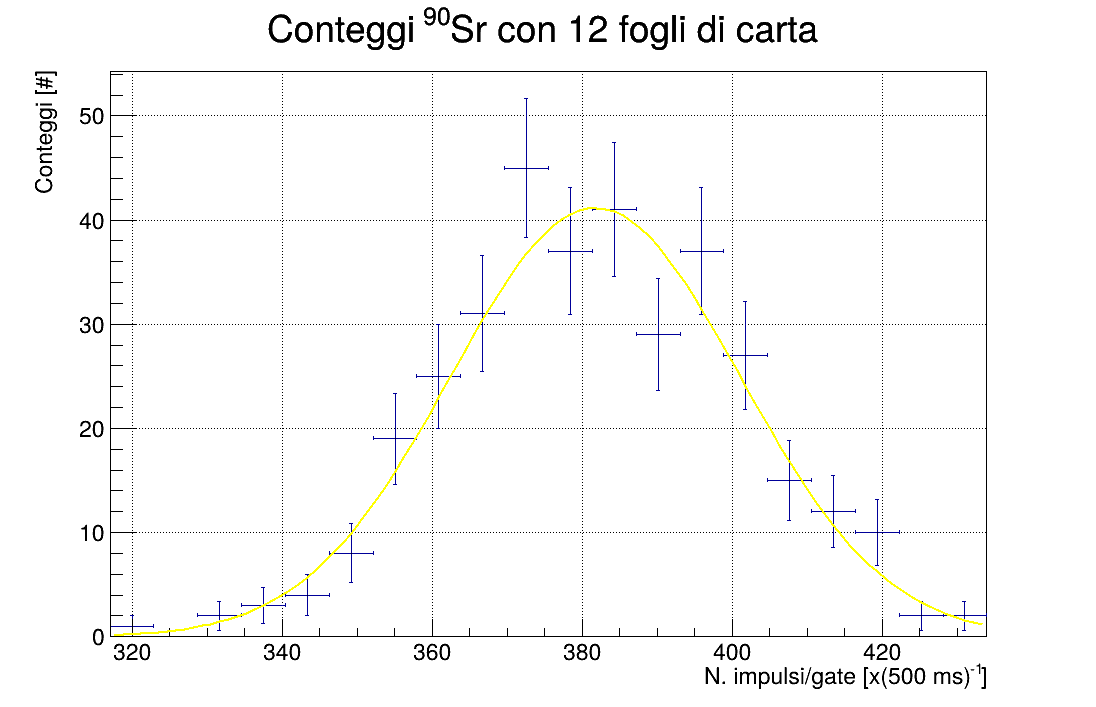
\includegraphics[width=0.99\linewidth]{appendice/carta/c4.png}
    \caption{\footnotesize $\chi^2=11$, d.o.f.$=16$}
     
\end{figure}
\begin{figure}[H]
    \centering
    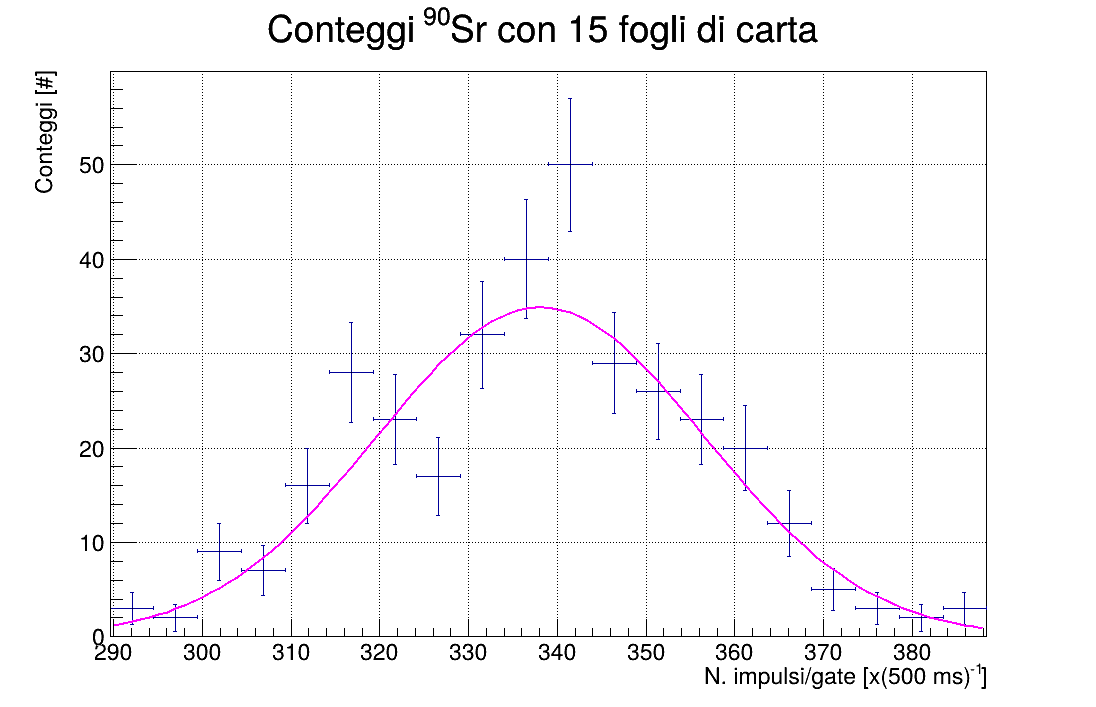
\includegraphics[width=0.99\linewidth]{appendice/carta/c5.png}
    \caption{\footnotesize $\chi^2=25$, d.o.f.$=17$}
     
\end{figure}
\end{multicols}
\newpage
\begin{multicols}{2}
    \begin{figure}[H]
    \centering
    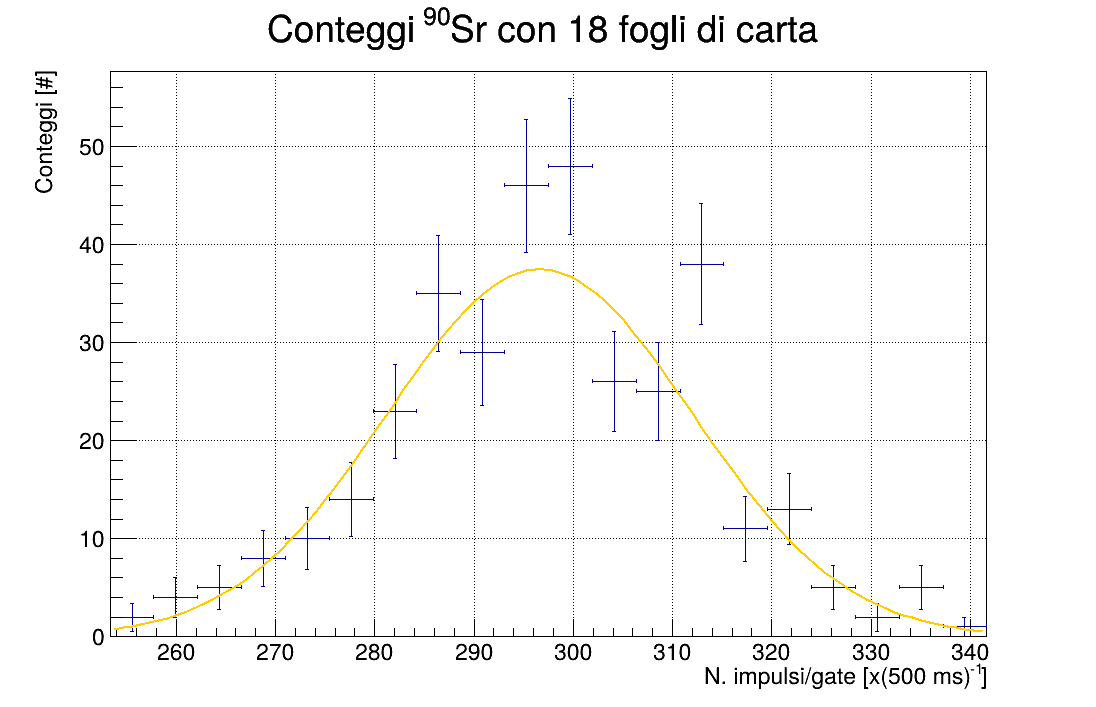
\includegraphics[width=0.99\linewidth]{appendice/carta/c6.png}
    \caption{\footnotesize $\chi^2=24$, d.o.f.$=17$}
     
\end{figure}
\begin{figure}[H]
    \centering
    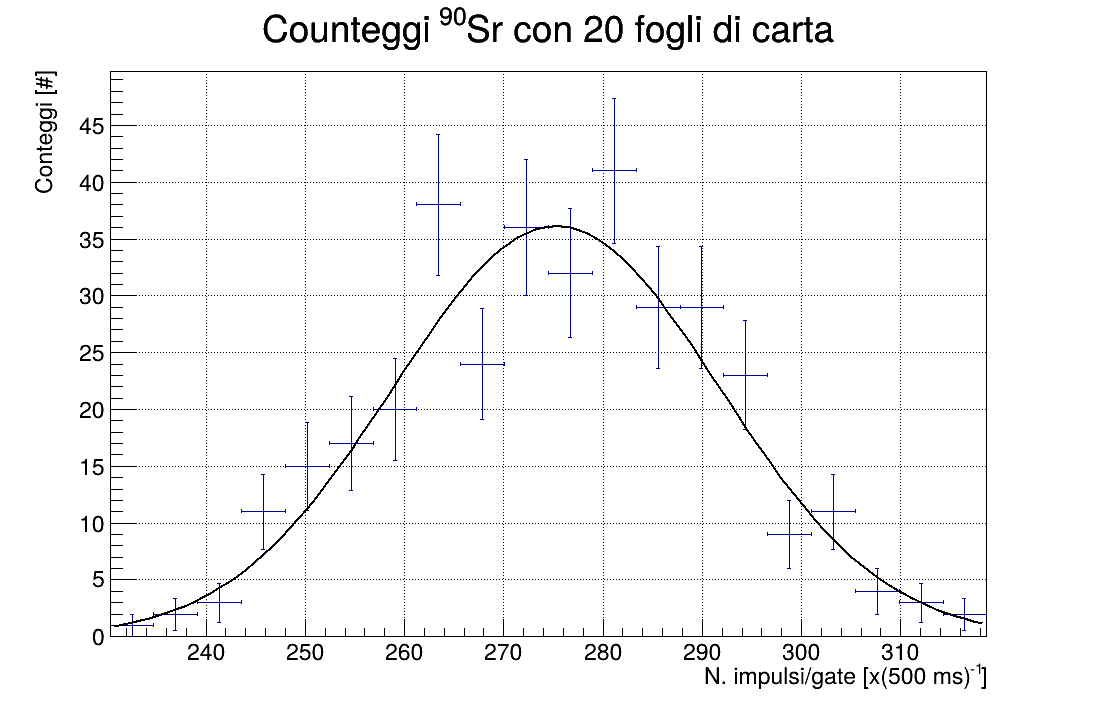
\includegraphics[width=0.99\linewidth]{appendice/carta/c7.png}
    \caption{\footnotesize $\chi^2=15$, d.o.f.$=17$}
     
\end{figure}
\end{multicols}

\subsubsection{Istogrammi per alluminio}

\begin{multicols}{2}
    \begin{figure}[H]
    \centering
    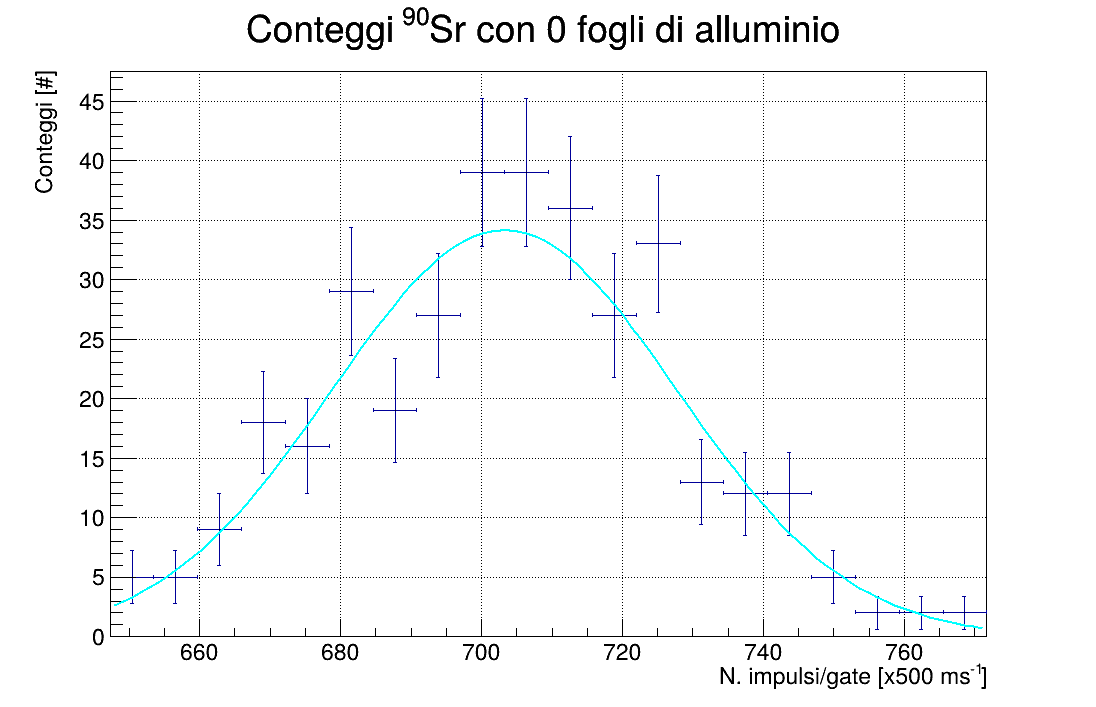
\includegraphics[width=0.99\linewidth]{appendice/alluminio/p0.png}
    \caption{\footnotesize $\chi^2=18$, d.o.f.$=17$}
     
\end{figure}
\begin{figure}[H]
    \centering
    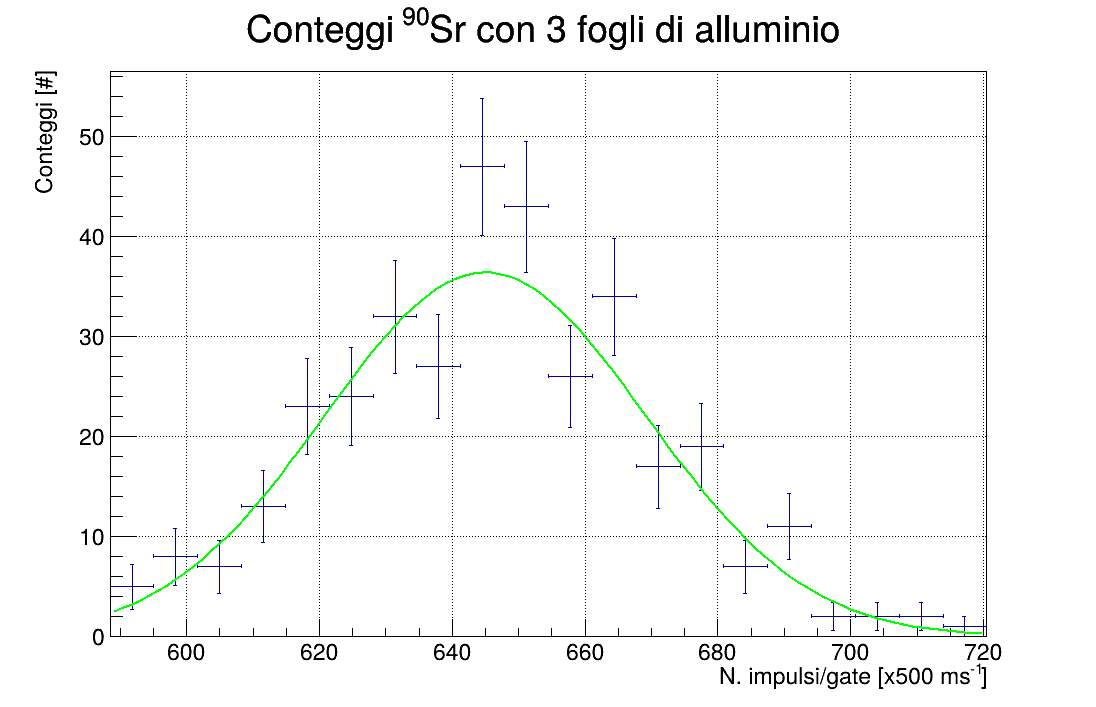
\includegraphics[width=0.99\linewidth]{appendice/alluminio/p1.png}
    \caption{\footnotesize $\chi^2=19$, d.o.f.$=17$}
     
\end{figure}
\end{multicols}
\begin{multicols}{2}
    \begin{figure}[H]
    \centering
    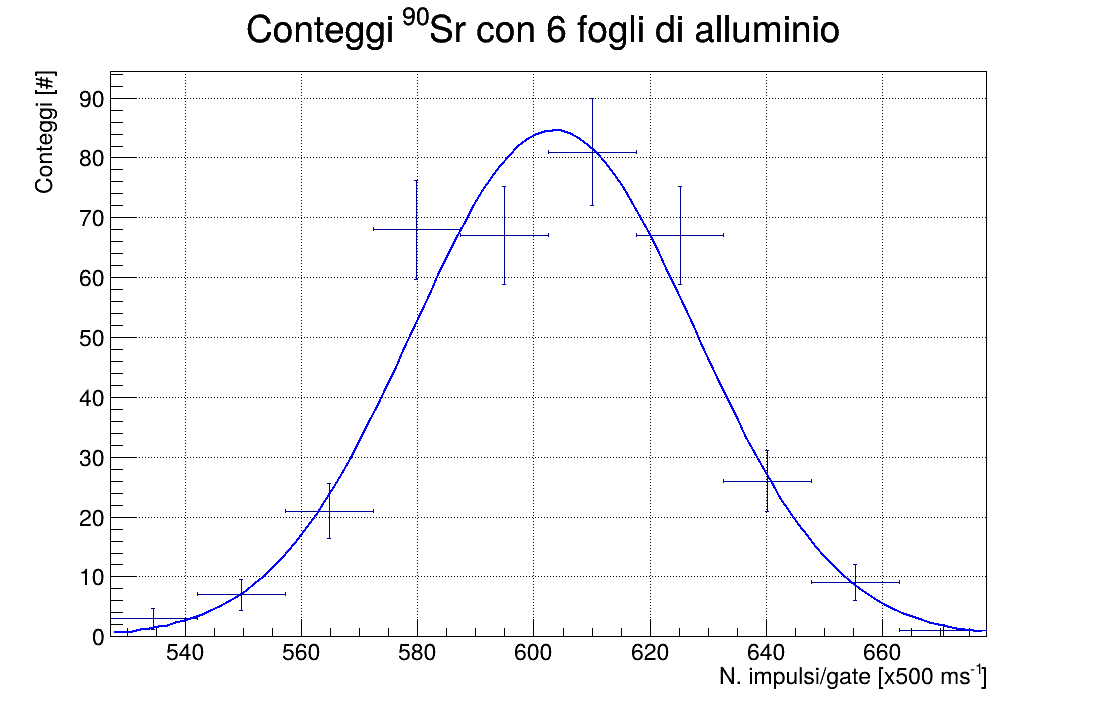
\includegraphics[width=0.99\linewidth]{appendice/alluminio/p2.png}
    \caption{\footnotesize $\chi^2=9$, d.o.f.$=7$}
     
\end{figure}
\begin{figure}[H]
    \centering
    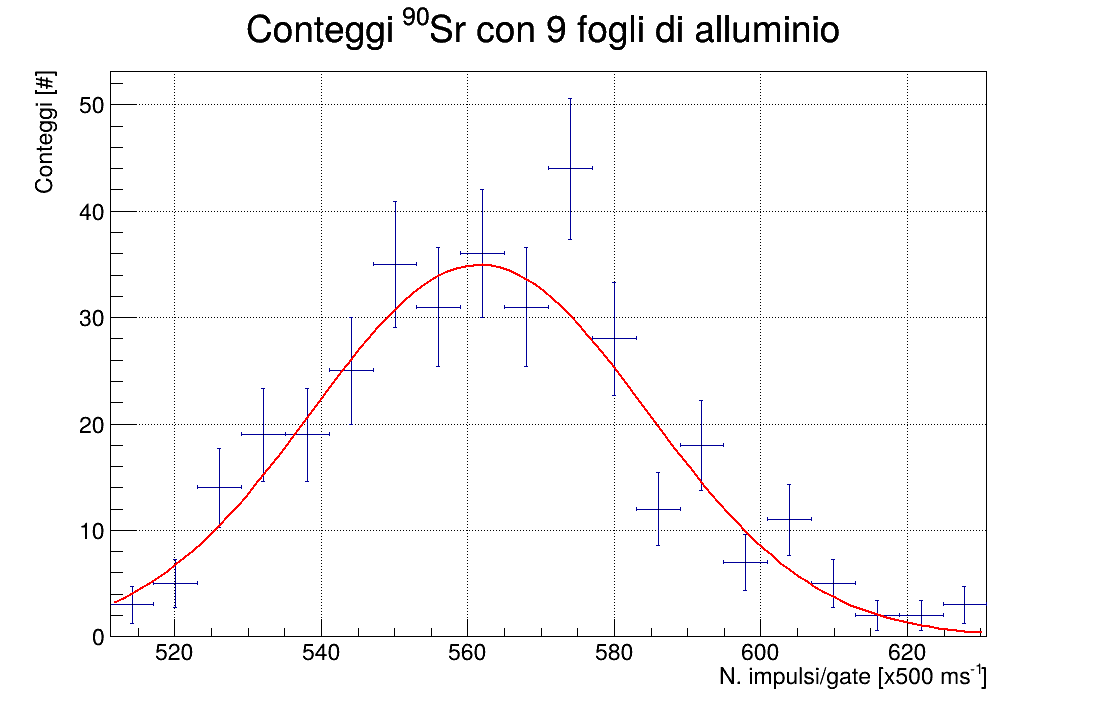
\includegraphics[width=0.99\linewidth]{appendice/alluminio/p3.png}
    \caption{\footnotesize $\chi^2=20$, d.o.f.$=17$}
     
\end{figure}
\end{multicols}
\newpage
\begin{multicols}{2}
    \begin{figure}[H]
    \centering
    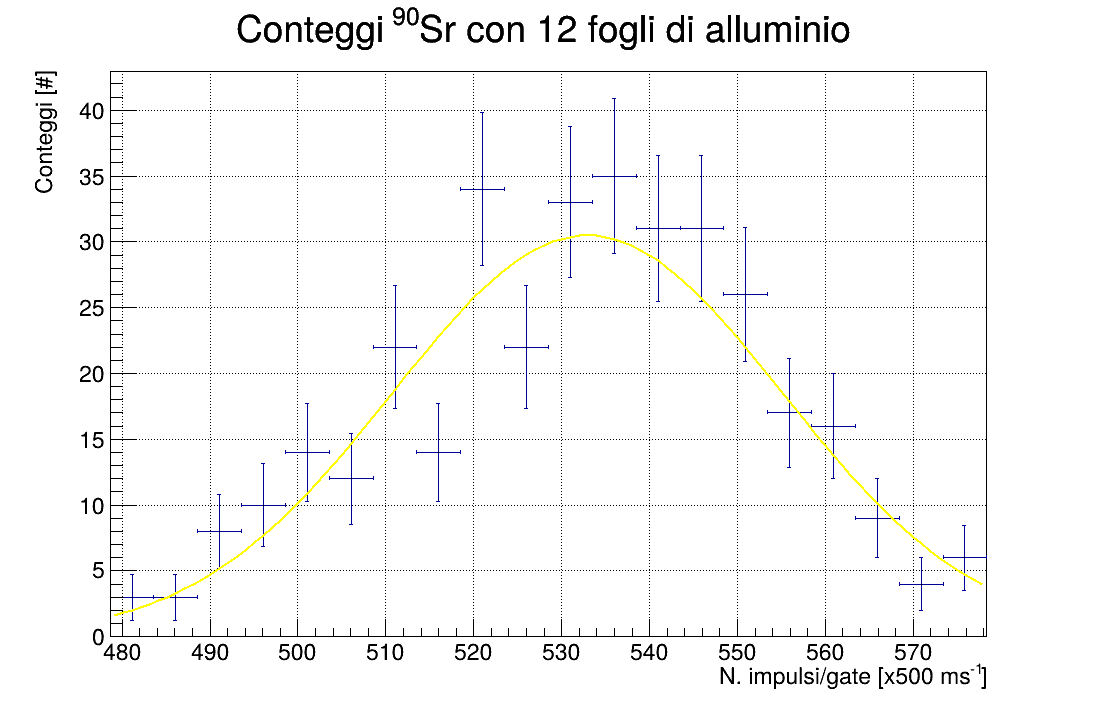
\includegraphics[width=0.99\linewidth]{appendice/alluminio/p4.png}
    \caption{\footnotesize $\chi^2=19$, d.o.f.$=17$}
     
\end{figure}
\begin{figure}[H]
    \centering
    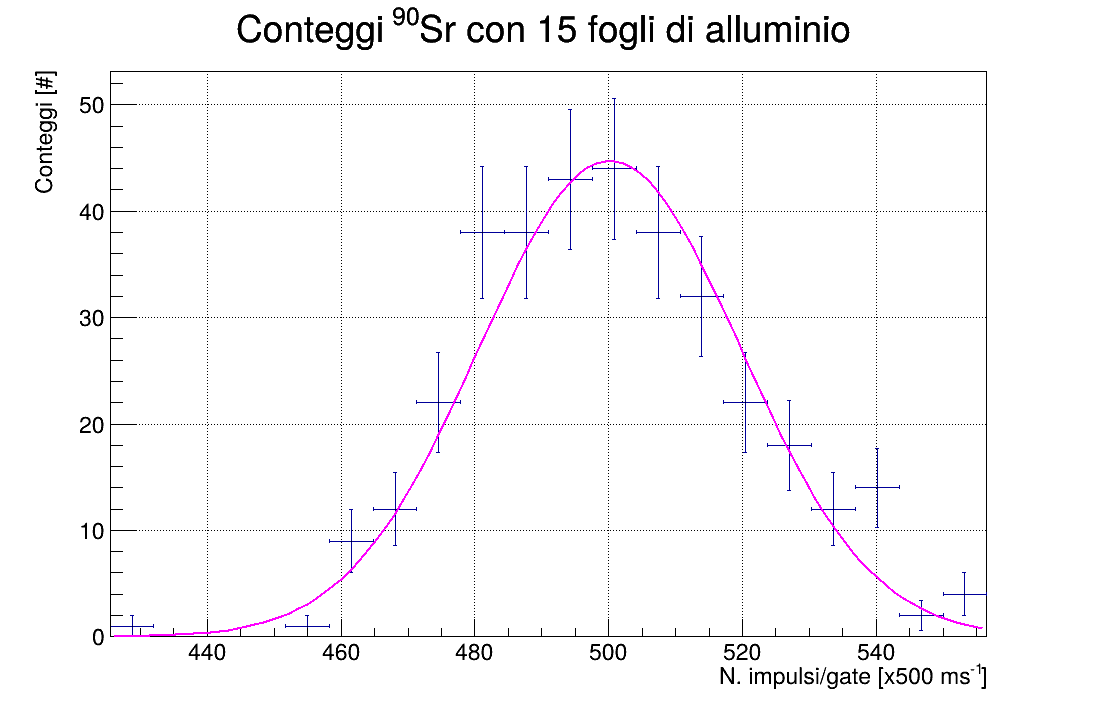
\includegraphics[width=0.99\linewidth]{appendice/alluminio/p5.png}
    \caption{\footnotesize $\chi^2=18$, d.o.f.$=14$}
     
\end{figure}
\end{multicols}


\begin{multicols}{2}
    \begin{figure}[H]
    \centering
    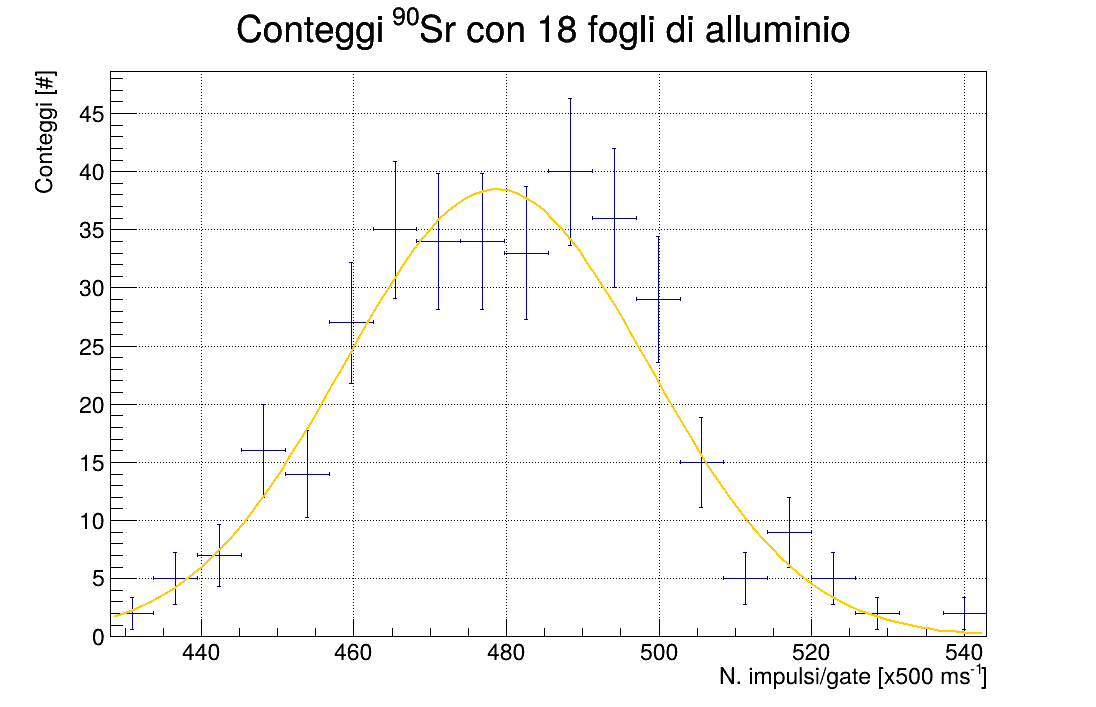
\includegraphics[width=0.99\linewidth]{appendice/alluminio/p6.png}
    \caption{\footnotesize $\chi^2=17$, d.o.f.$=16$}
     
\end{figure}
\begin{figure}[H]
    \centering
    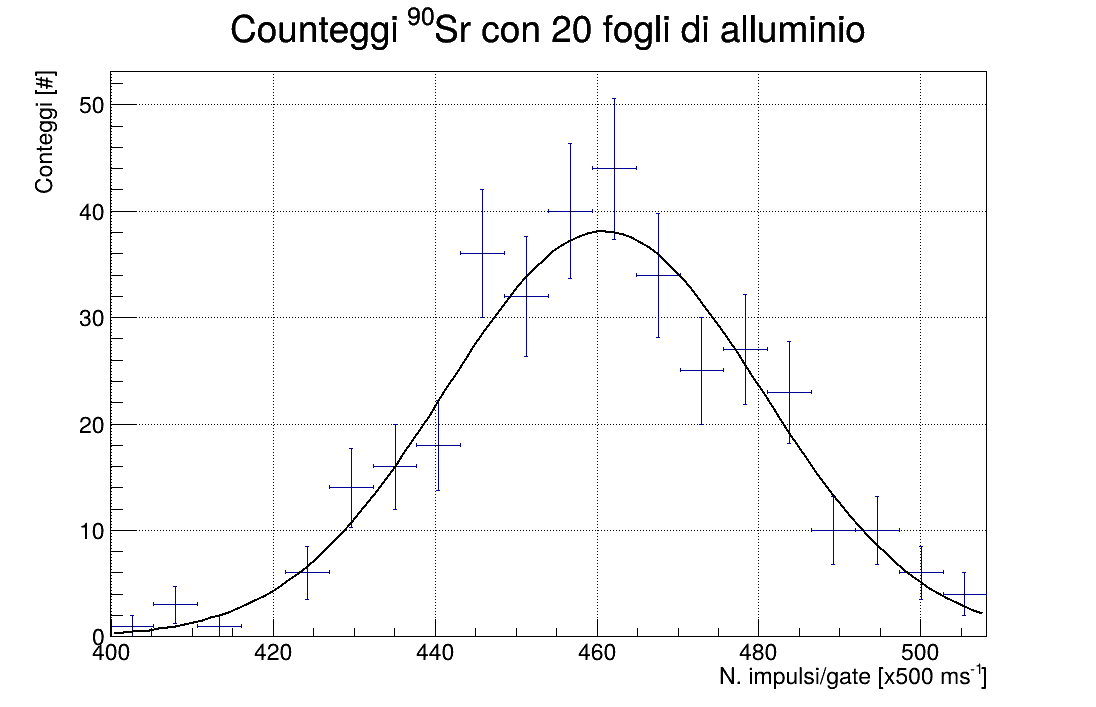
\includegraphics[width=0.99\linewidth]{appendice/alluminio/p7.png}
    \caption{\footnotesize $\chi^2=11$, d.o.f.$=16$}
     
\end{figure}
\end{multicols}

\subsection{Picco di conversione interna del ${}^{137}$Cs}

Si riportano i parametri del fit del picco di conversione interna: i pedici $1$ sono riferiti all'andamento decrescente dello spettro, mentre quelli $2$ al picco di conversione interna.
$$y = N_1 \exp\left\{-\frac{(x-\mu_1)^2}{2\sigma_1^2}\right\} + N_2 \exp\left\{-\frac{(x-\mu_2)^2}{2\sigma_2^2}\right\}$$

\begin{table}[H]
    \centering
    \begin{tabular}{|c|c|c|c|c|c|c|c|}
    \hline
    $\mathbf{N_1 [\#]}$ & $\mathbf{\mu_1}$\textbf{[CHN]} & $\mathbf{\sigma_1}$\textbf{[CHN]} &
    $\mathbf{N_2 [\#]}$ & $\mathbf{\mu_2}$\textbf{[CHN]} & $\mathbf{\sigma_2}$\textbf{[CHN]} & $\mathbf{\chi^2}$ & \textbf{d.o.f.}\\
    \hline
    $9700\pm1600$ & $-3300\pm1200$ & $8400\pm300$ & $719\pm6$ & $19700\pm30$ & $251\pm20$ & 325 & 286 \\
    \hline
    \end{tabular}
\end{table}
\newpage
\subsection{Stima di $\langle \Delta_{pp}\rangle$ per lo spettro del ${}^{137}$Cs}

Si riportano qui i valori dei picchi della sezione 2.3.3, le loro incertezze e le stime di $\Delta_{pp}$.

\begin{table}[H]
    \centering
    \begin{tabular}{|c|c|c|c|c|}
        \hline
        
        \textbf{N. picco} & \textbf{$\mathbf{\chi^2}$ fit} & \textbf{d.o.f.} &$\mathbf{(p_i\pm\sigma_{p,i})\cdot10}$\textbf{[CHN]} & $\mathbf{\Delta_{pp}\cdot10}$\textbf{[CHN]} \\ \hline
        1   & 8 & 8 & $143\pm5$    & \textbf{X} \\ \hline
        2   & 4 & 5 & $160\pm4$    & $17\pm6$ \\ \hline        
        3   & 11 & 6 & $178\pm5$  & $17\pm7$ \\ \hline
        4   & 16 & 8 & $195\pm6$   & $17\pm7$ \\ \hline
        5   & 13 & 9 & $213\pm6$ & $18\pm8$ \\ \hline
        6   & 9 & 9 & $230\pm 7$ & $17\pm9$ \\ \hline
        7   & 11 & 7 & $248\pm6$ & $18\pm9$ \\ \hline
        8   & 6 & 7 & $266\pm6$ & $17\pm9$ \\ \hline
        9   & 10 & 8 & $283\pm7$ & $17\pm10$ \\ \hline
        10   & 5 & 7 & $300\pm7$ & $17\pm10$ \\ \hline
    \end{tabular}
    \caption{\footnotesize Coordinate dei picchi, parametri dei fit e stime di $\Delta_{pp}$ utilizzate per il calcolo di $\langle\Delta_{pp}\rangle$ .}
    \label{tab:zoomcs}   
\end{table}

